\documentclass[compress]{beamer}
\usepackage{ifthen,verbatim,ulem}

\newcommand{\isnote}{}
\xdefinecolor{lightyellow}{rgb}{1.,1.,0.25}
\xdefinecolor{darkblue}{rgb}{0.1,0.1,0.7}

%% Uncomment this to get annotations
%% \def\notes{\addtocounter{page}{-1}
%%            \renewcommand{\isnote}{*}
%% 	   \beamertemplateshadingbackground{lightyellow}{white}
%%            \begin{frame}
%%            \frametitle{Notes for the previous page (page \insertpagenumber)}
%%            \itemize}
%% \def\endnotes{\enditemize
%% 	      \end{frame}
%%               \beamertemplateshadingbackground{white}{white}
%%               \renewcommand{\isnote}{}}

%% Uncomment this to not get annotations
\def\notes{\comment}
\def\endnotes{\endcomment}

\setbeamertemplate{navigation symbols}{}
\setbeamertemplate{headline}{\mbox{ } \hfill
\begin{minipage}{5.5 cm}
\vspace{-0.75 cm} \small
\end{minipage} \hfill
\begin{minipage}{4.5 cm}
\vspace{-0.75 cm} \small
\begin{flushright}
\ifthenelse{\equal{\insertpagenumber}{1}}{}{Jim Pivarski \hspace{0.2 cm} \insertpagenumber\isnote/\pageref{numpages}}
\end{flushright}
\end{minipage}\mbox{\hspace{0.2 cm}}\includegraphics[height=1 cm]{../cmslogo} \hspace{0.1 cm} \includegraphics[height=1 cm]{../tamulogo} \hspace{0.01 cm} \vspace{-1.05 cm}}

\begin{document}
\begin{frame}
\vfill
\begin{center}
\textcolor{darkblue}{\Large Track-based CSC Alignment and}

\vspace{0.2 cm}
\textcolor{darkblue}{\Large Global CMS Alignment}

\vfill
\begin{columns}
\column{0.3\linewidth}
\begin{center}
\large
Jim Pivarski
\end{center}
\end{columns}

\begin{columns}
\column{0.3\linewidth}
\begin{center}
\scriptsize
{\it Texas A\&M University}
\end{center}
\end{columns}

\vfill
 9 December, 2008

\end{center}
\end{frame}

%% \begin{notes}
%% \item This is the annotated version of my talk.
%% \item If you want the version that I am presenting, download the one
%% labeled ``slides'' on Indico (or just ignore these yellow pages).
%% \item The annotated version is provided for extra detail and a written
%% record of comments that I intend to make orally.
%% \item Yellow notes refer to the content on the {\it previous} page.
%% \item All other slides are identical for the two versions.
%% \end{notes}

\small

\begin{frame}
\frametitle{Introduction}
\begin{itemize}\setlength{\itemsep}{0.5 cm}
\item \textcolor{darkblue}{CSC Alignment:} chambers within rings
\begin{itemize}
\item achieved target resolution of 300~$\mu$m
\end{itemize}

\item layers within chambers
\begin{itemize}
\item early plots show small misalignments
\end{itemize}

\item \textcolor{darkblue}{Global CMS alignment:} wheels and disks relative to tracker
\begin{itemize}\setlength{\itemsep}{0.1 cm}
\item produced muon alignment constants, but results are surprising
\item sensitivity to tracker could constrain tracker alignment
\end{itemize}
\end{itemize}
%% \hspace{-0.83 cm} \textcolor{darkblue}{\Large Outline2}
\end{frame}

%% \section*{First section}
%% \begin{frame}
%% \begin{center}
%% \Huge \textcolor{blue}{First section}
%% \end{center}
%% \end{frame}

\begin{frame}
\frametitle{CSC Alignment}
\begin{itemize}
\item Muon chambers can be individually aligned to the tracker with 10--100~pb$^{-1}$ of globalMuons
\item But for CSCs, it will require much less data to
\begin{enumerate}
\item align chambers relative to each other \hfill \textcolor{darkblue}{Overlaps procedure} \\ in each ring
\item align the ring to the tracker \hfill \textcolor{darkblue}{globalMuon procedure}
\end{enumerate}
\end{itemize}

\begin{columns}
\column{0.5\linewidth}
\textcolor{darkblue}{Overlaps procedure:}
\begin{enumerate}\setlength{\itemsep}{0 cm}
\item select tracks that pass through overlap of two CSCs
\item require consistency in pair of segments: slope and intercept
\item solve system for all pairs
\end{enumerate}

\column{0.2\linewidth}
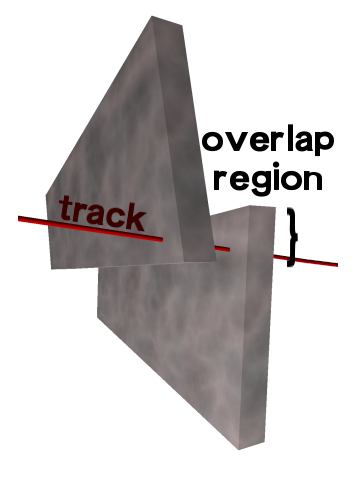
\includegraphics[width=\linewidth]{overlaps.png}

\column{0.3\linewidth}
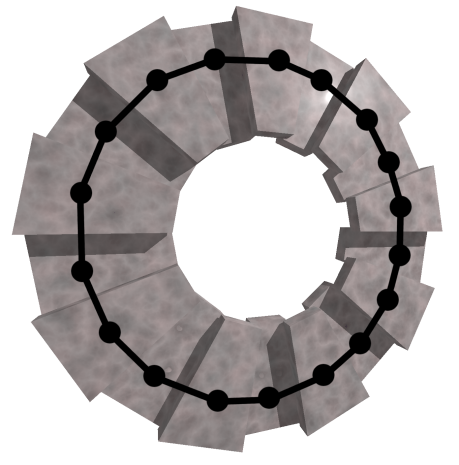
\includegraphics[width=\linewidth]{one_station.png}
\end{columns}

\vfill
\begin{itemize}
\item System is over-constrained: circle can't have any gaps!
\end{itemize}
\end{frame}

\begin{frame}
\frametitle{CSC Overlaps alignment results}
\begin{columns}
\column{0.4\linewidth}

ME$-$2/1 and $-$3/1 (most complete in \mbox{beam-halo dataset)\hspace{-1 cm}}

\begin{itemize}
\item Expect $\sim$230~$\mu$m resolution in $r\phi$ (MC)

\item Alignment results in data follow photogrammetry (PG) measurement

\item Alignment resolution from PG comparison: \\ \mbox{ } \hfill 270~$\mu$m \hfill \hfill \mbox{ }

\item Similarly, $\phi_z$ resolution is 0.35~mrad

\item {\it Minutes} of beam-halo \mbox{data!\hspace{-1 cm}}
\end{itemize}

\vspace{0.2 cm}
\tiny Pivarski, Safonov (Texas A\&M), \mbox{Banicz (US-CMS)\hspace{-1 cm}}

\column{0.66\linewidth}

\vspace{0.2 cm}
\mbox{ } \hfill data: aligned (histogram) and PG \textcolor{blue}{(data)} \hfill \mbox{ }
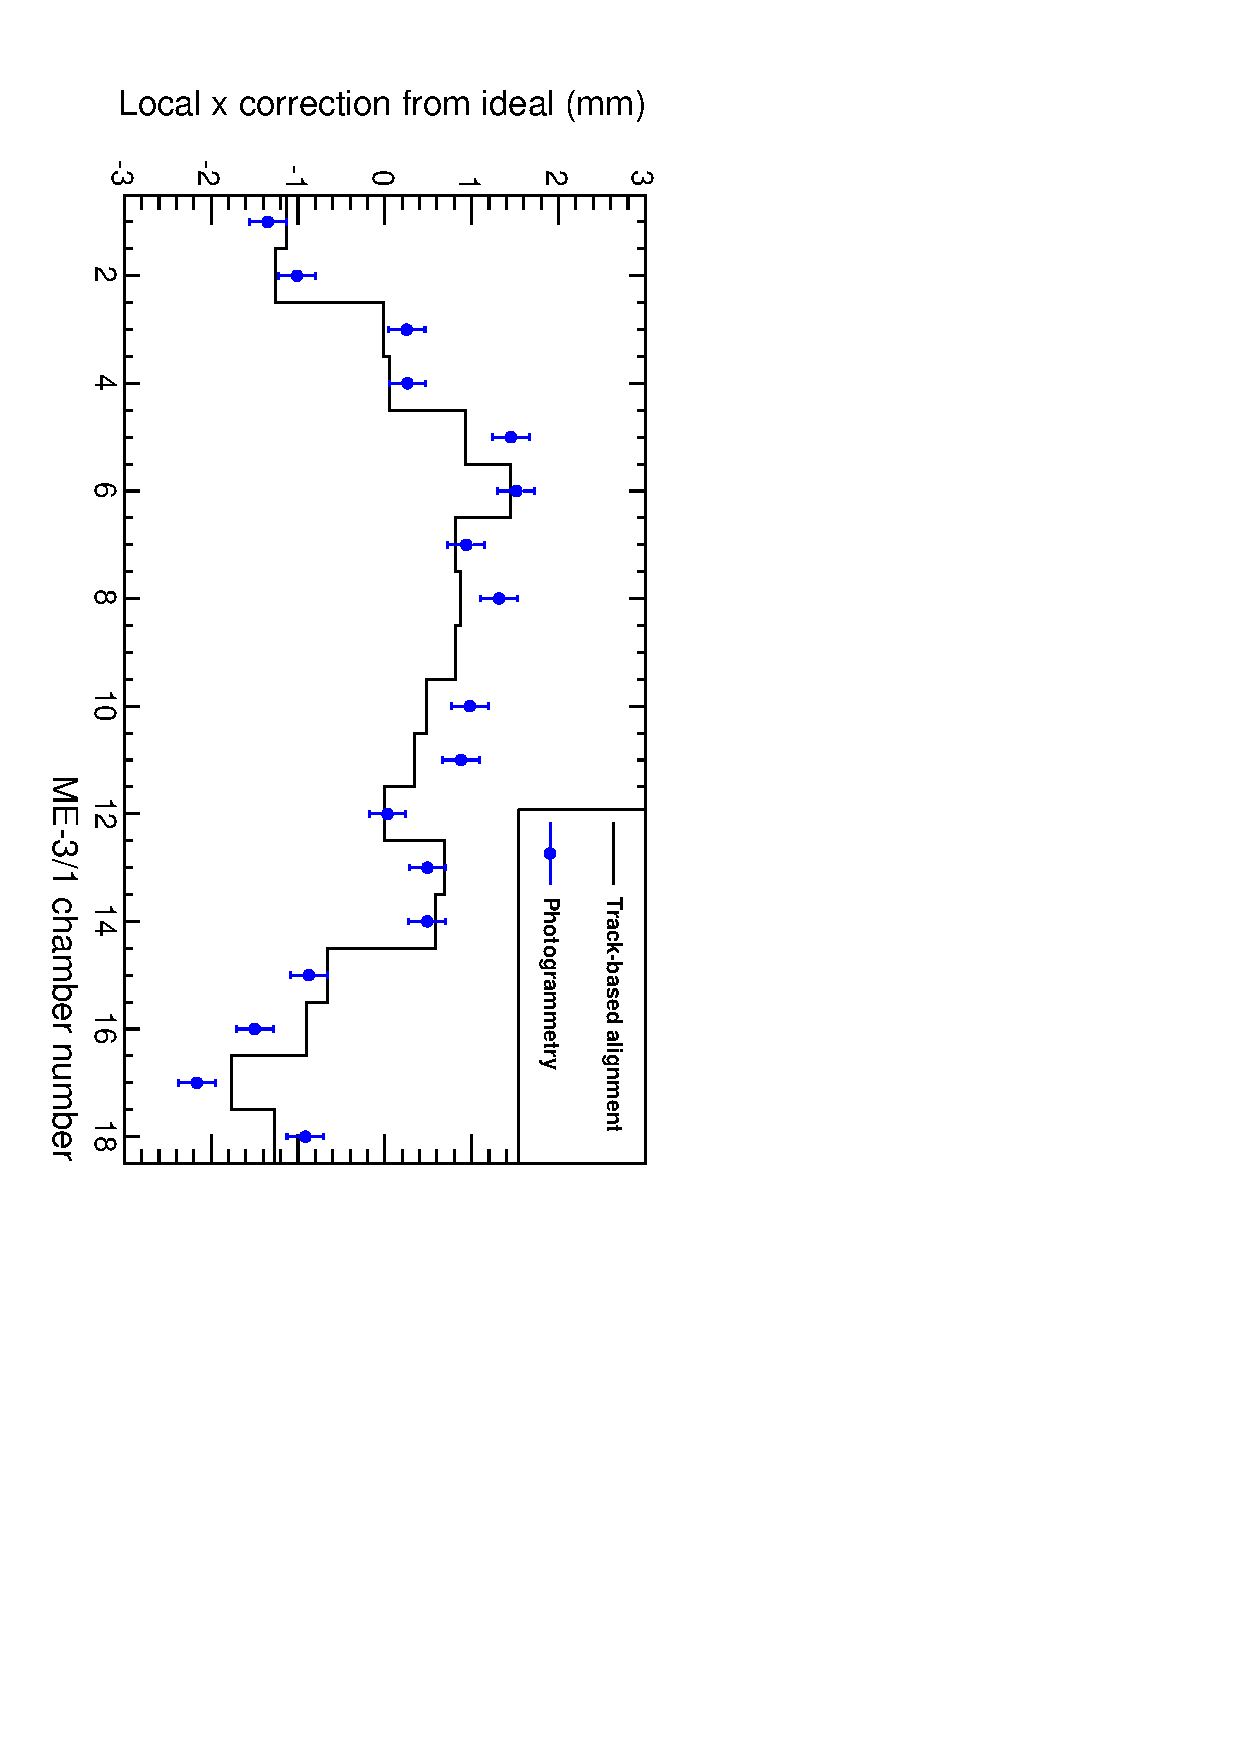
\includegraphics[height=\linewidth, angle=90]{compare_m31_x.pdf}

\vspace{0.2 cm}
\begin{tabular}{c c}
MC: aligned - truth & data: aligned - PG \\
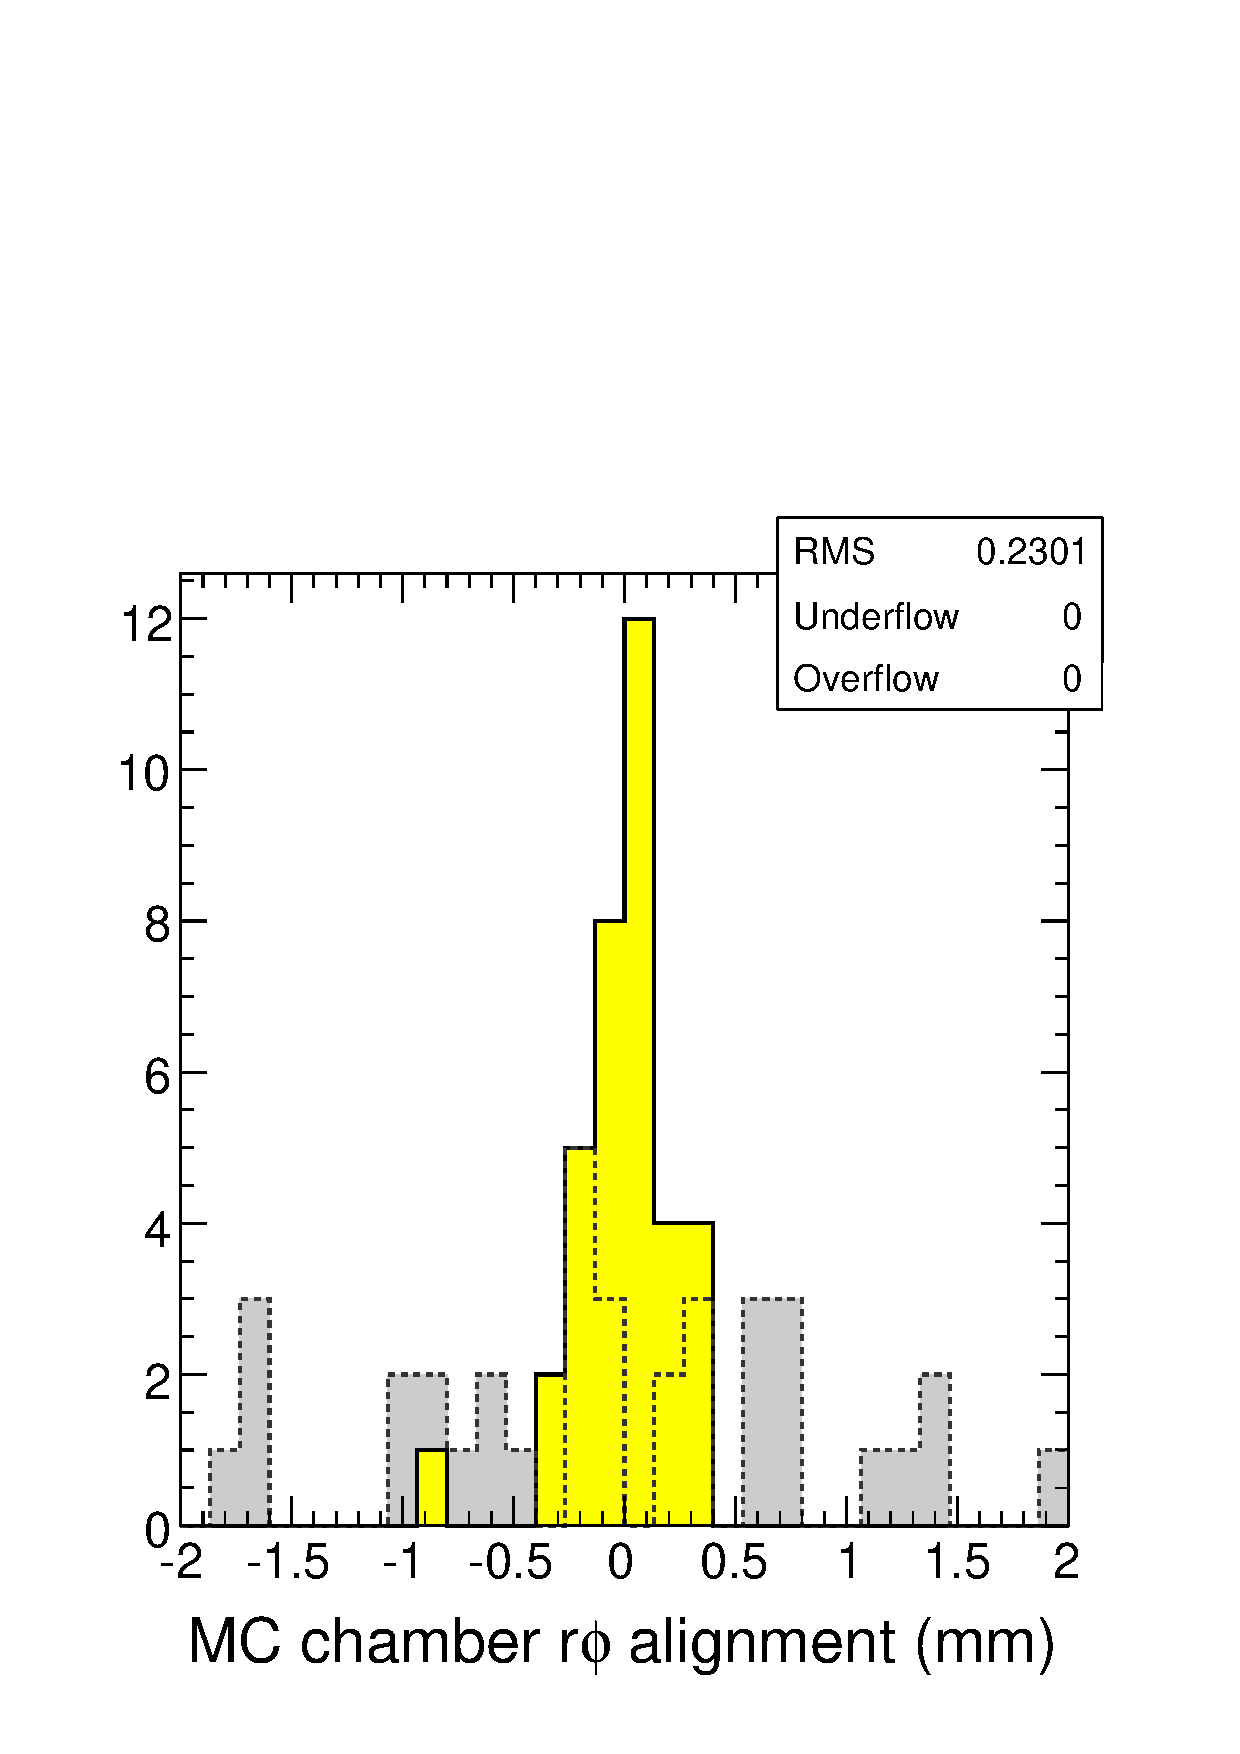
\includegraphics[width=0.45\linewidth]{mcchamber_rphi.pdf} &
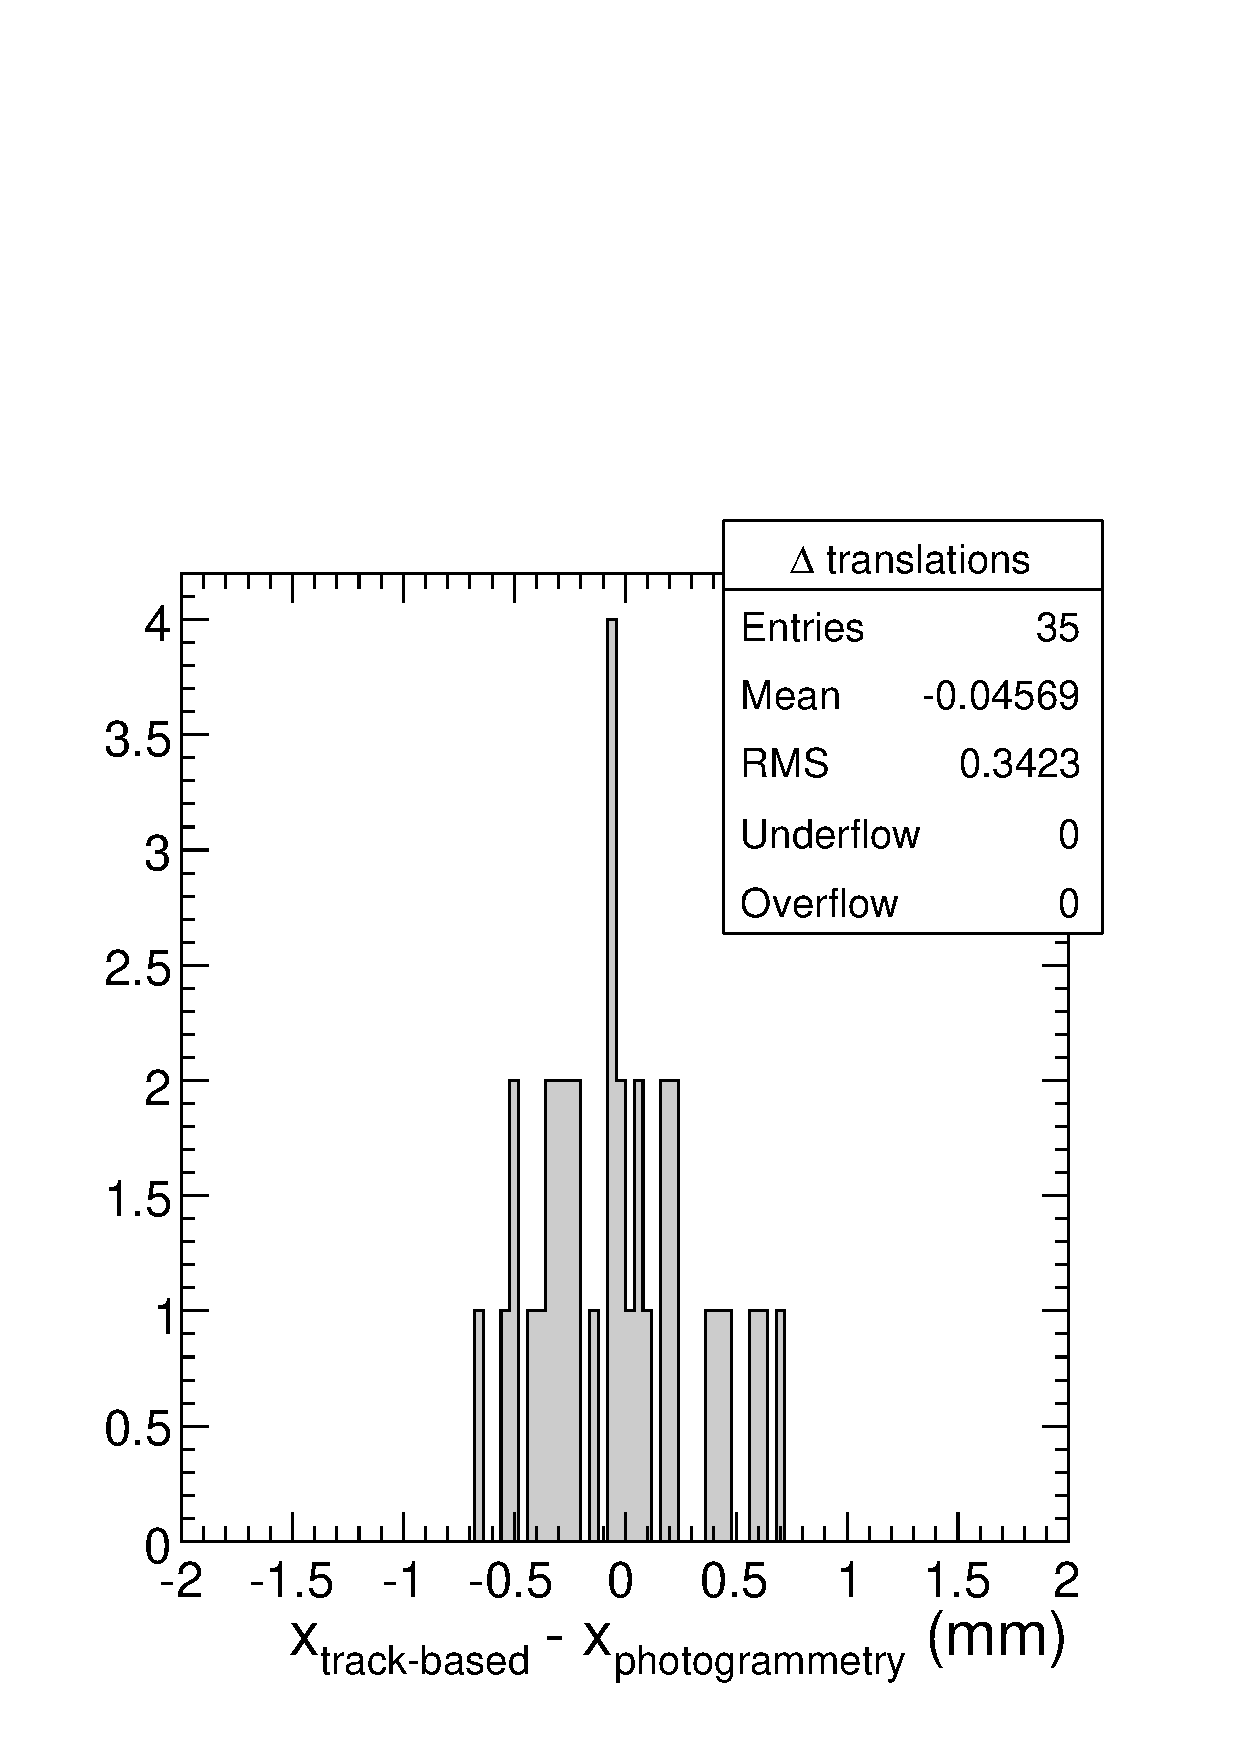
\includegraphics[width=0.45\linewidth]{delta_translations.pdf}
\end{tabular}
\end{columns}
\end{frame}

\begin{frame}
\frametitle{Closure constraint}
\begin{itemize}\setlength{\itemsep}{0.25 cm}
\item Each residual is a difference of positions of neighbors $(x_i - x_{i+1})$
\item Must sum to zero: $(x_1 - x_2) + (x_2 - x_3) + \ldots + (x_N - x_1) = 0$
\item $r\phi$ residuals summed to zero in MC, but not data
\item Precision agreement with photogrammetry is only possible if this
  is due to a uniform error in the chamber description:
\begin{itemize}
\item {\it either} chamber active volume is 2.5~mm closer to beamline
\item {\it or} width of active volume is wrong by 800~$\mu$m
\item (or a little of both, or something equivalent)
\end{itemize}
\item \textcolor{darkblue}{Resolution:} CSC strip pitch angle in CMSSW
  was set to \mbox{design value,\hspace{-0.25 cm}} rather than the measurement: a 10~$\mu$m width
  error $\times$ 80~strips
\end{itemize}
\begin{center}
\hspace{-1 cm} $\displaystyle \sum_{\mbox{\scriptsize chambers }i} (r_i - r_{i+1}) = \bigg\{$
\begin{tabular}{c c c}
& with design pitch & with real pitch \\\hline
ME$-$2/1 & $+$14.30~mm & -0.72 $\pm$ 0.42~mm \\
ME$-$3/1 & $+$15.90~mm & -0.36 $\pm$ 0.51~mm \\
\end{tabular}
\end{center}
\end{frame}

\begin{frame}
\frametitle{Early look at CSC layer alignment}
\begin{columns}
\column{0.4\linewidth}
\begin{itemize}
\item CSC overlaps region has 12~hits $-$ 2~to \mbox{determine\hspace{-0.5 cm}} track = 5~unbiased hits per chamber

\item 5/6~layers is a complete internal alignment

\item Test in MC (middle): residuals reproduce test-pattern {\scriptsize (high stats)}

\item Plot from data \mbox{(bottom):\hspace{-0.5 cm}} typical misalignment 100--200~$\mu$m

\item Need 9~minutes $\times$ $10^2$ for high precision  :)

\end{itemize}

\vspace{0.5 cm}
\tiny Pivarski, Safonov (Texas A\&M), \mbox{Banicz (US-CMS)\hspace{-1 cm}}

\column{0.6\linewidth}
\vspace{0.5 cm}
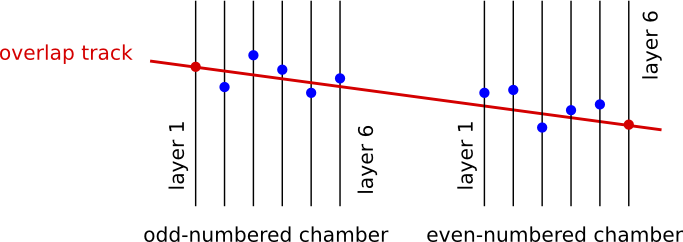
\includegraphics[width=\linewidth]{layer_alignment_noskew.png}

\vspace{0.2 cm}
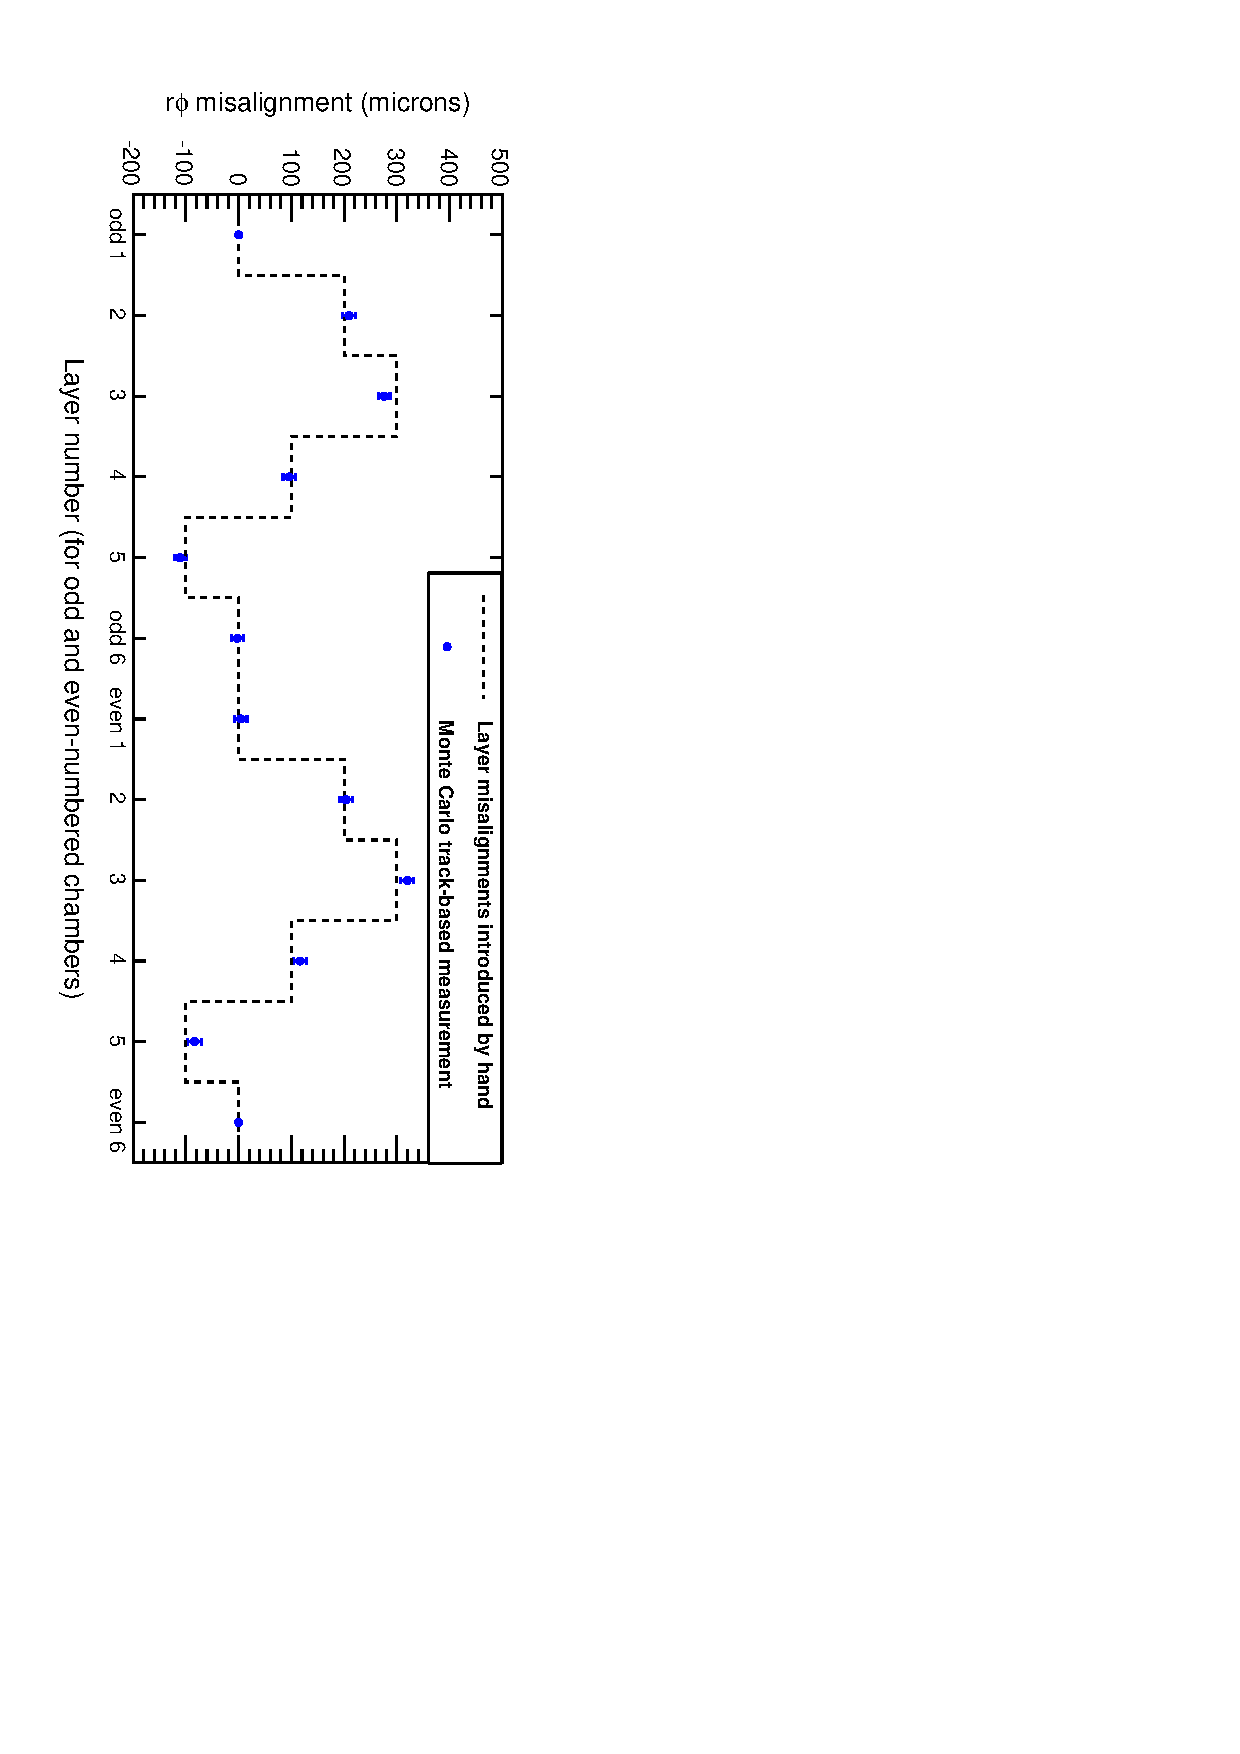
\includegraphics[height=\linewidth, angle=90]{layer_test.pdf}

\vspace{0.2 cm}
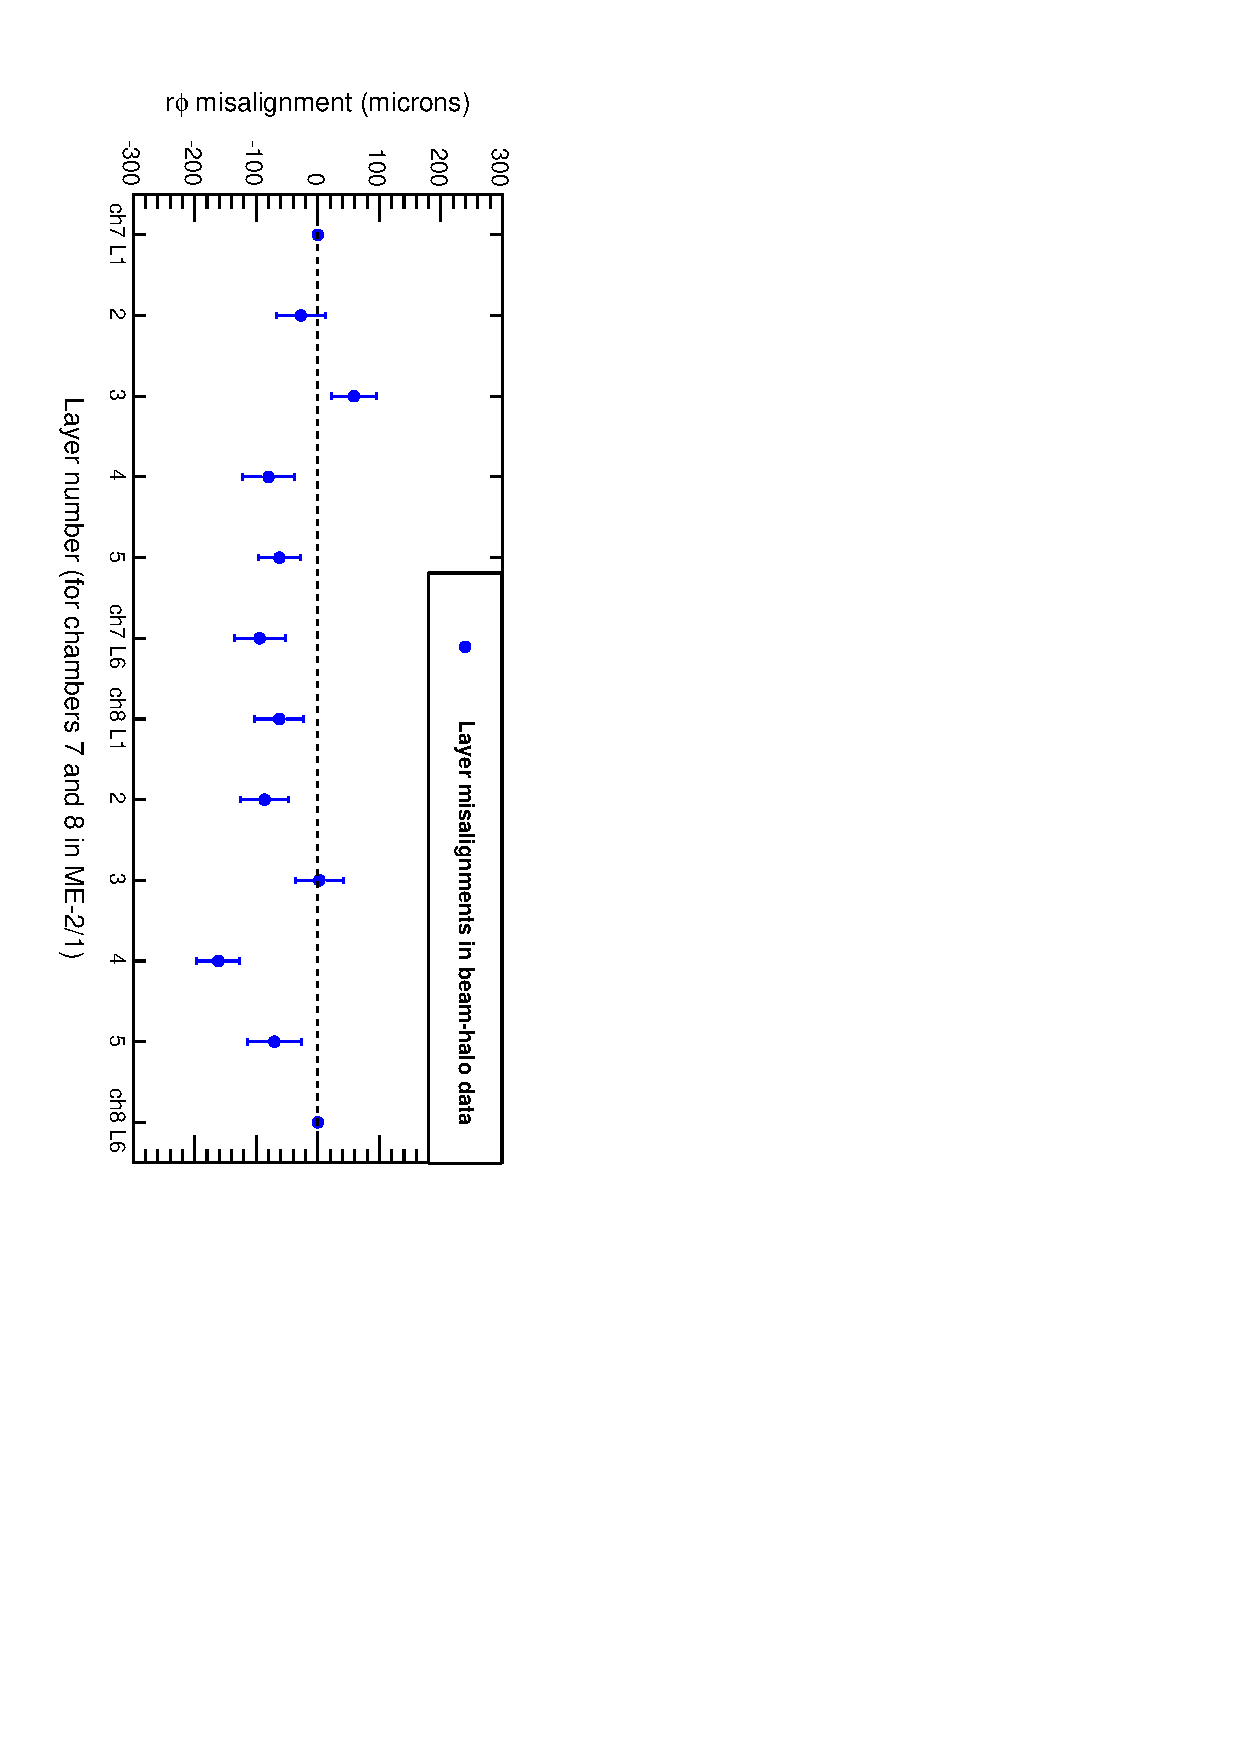
\includegraphics[height=\linewidth, angle=90]{layer_data.pdf}
\end{columns}
\end{frame}

\begin{frame}
\frametitle{Global muon alignment}

\begin{columns}
\column{0.5\linewidth}
\begin{itemize}
\item Alignment of muon system relative to tracker:
\begin{itemize}\setlength{\itemsep}{0.05 cm}
\item select globalMuon tracks by momentum
\item refit, ignoring muon hits
\item use unbiased residuals to align wheels/disks
\end{itemize}
\end{itemize}

\column{0.6\linewidth}
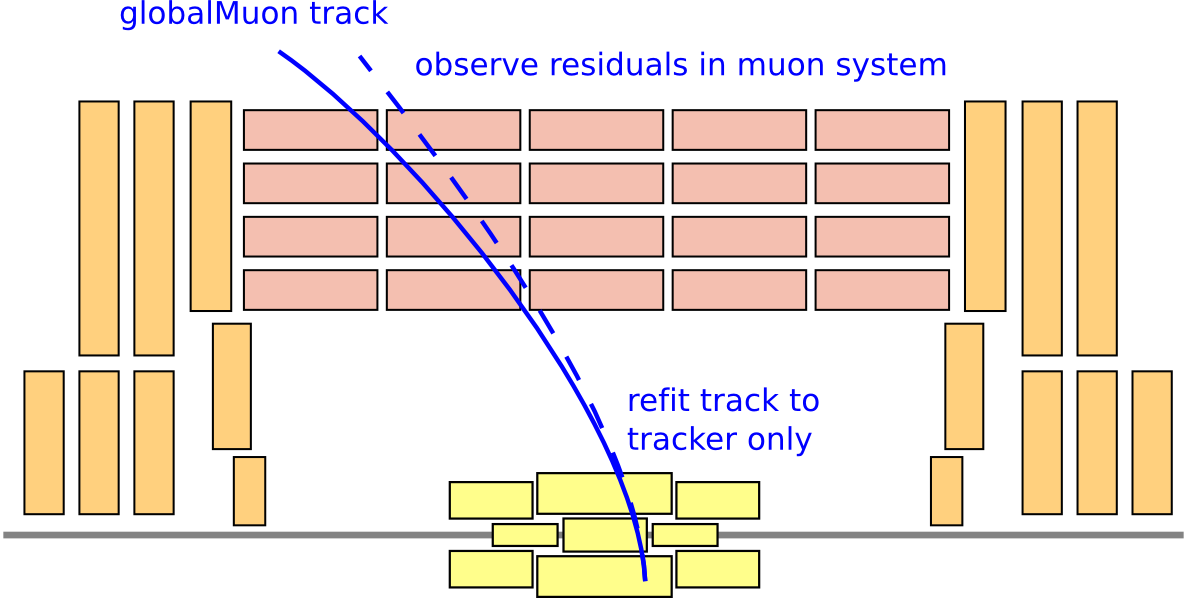
\includegraphics[width=\linewidth]{globalMuons.png}
\end{columns}

\begin{columns}
\column{1.12\linewidth}
\begin{itemize}
\item Same procedure can later be applied to individual chambers
\begin{itemize}
\item Wheel/disk alignment is both ``practice'' and the largest part of the alignment correction
\end{itemize}
\item Both HIP and MillePede groups used procedures like this\ldots
\begin{itemize}
\item which roughly agreed with each other (6 d.o.f.)
\item in time for CRAFT re-processing
\item but they had unexpected features: twist around beamline ($d\phi_z/dz$) \\ and $z$ expansion
\end{itemize}
\item Not used in this round of re-processing
\end{itemize}
\end{columns}
\end{frame}

\begin{frame}
\frametitle{Momentum cut/extrapolation}

\begin{columns}
\column{0.6\linewidth}
\begin{itemize}
\item $\vec{B}$-field errors and multiple scattering affect low-momentum tracks
\item Alignment error $\to$ 0 as $|p| \to \infty$
\item Plot vs.\ curvature ($q/p_T$), fit around 0

\vspace{-0.2 cm}
\begin{itemize}
\item constant = misalignment
\item antisymmetric in $q$ = $\vec{B}$ errors
\item symmetric in $q$ = scattering
\end{itemize}
\end{itemize}

\vfill
\begin{columns}
\column{0.5\linewidth}
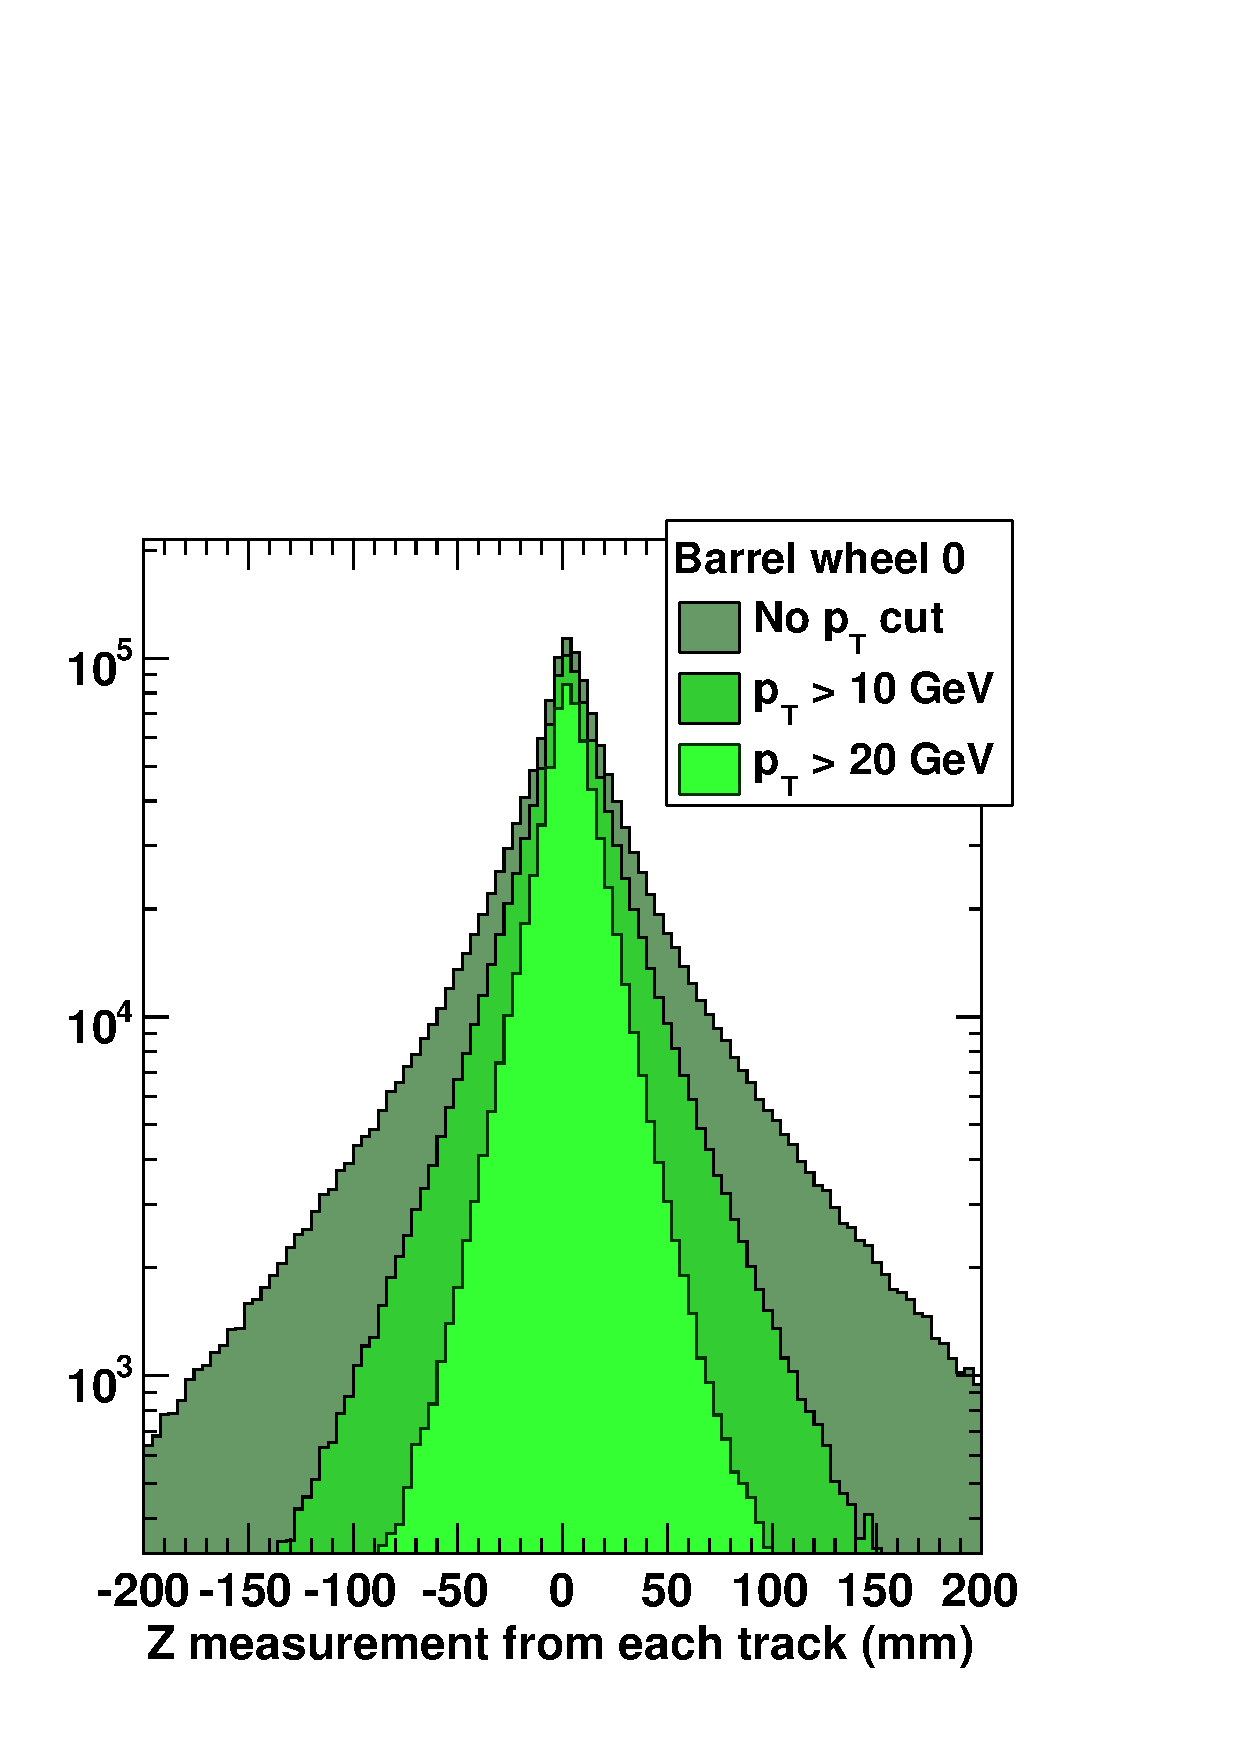
\includegraphics[width=\linewidth]{residuals_barrel.pdf}
\column{0.58\linewidth}
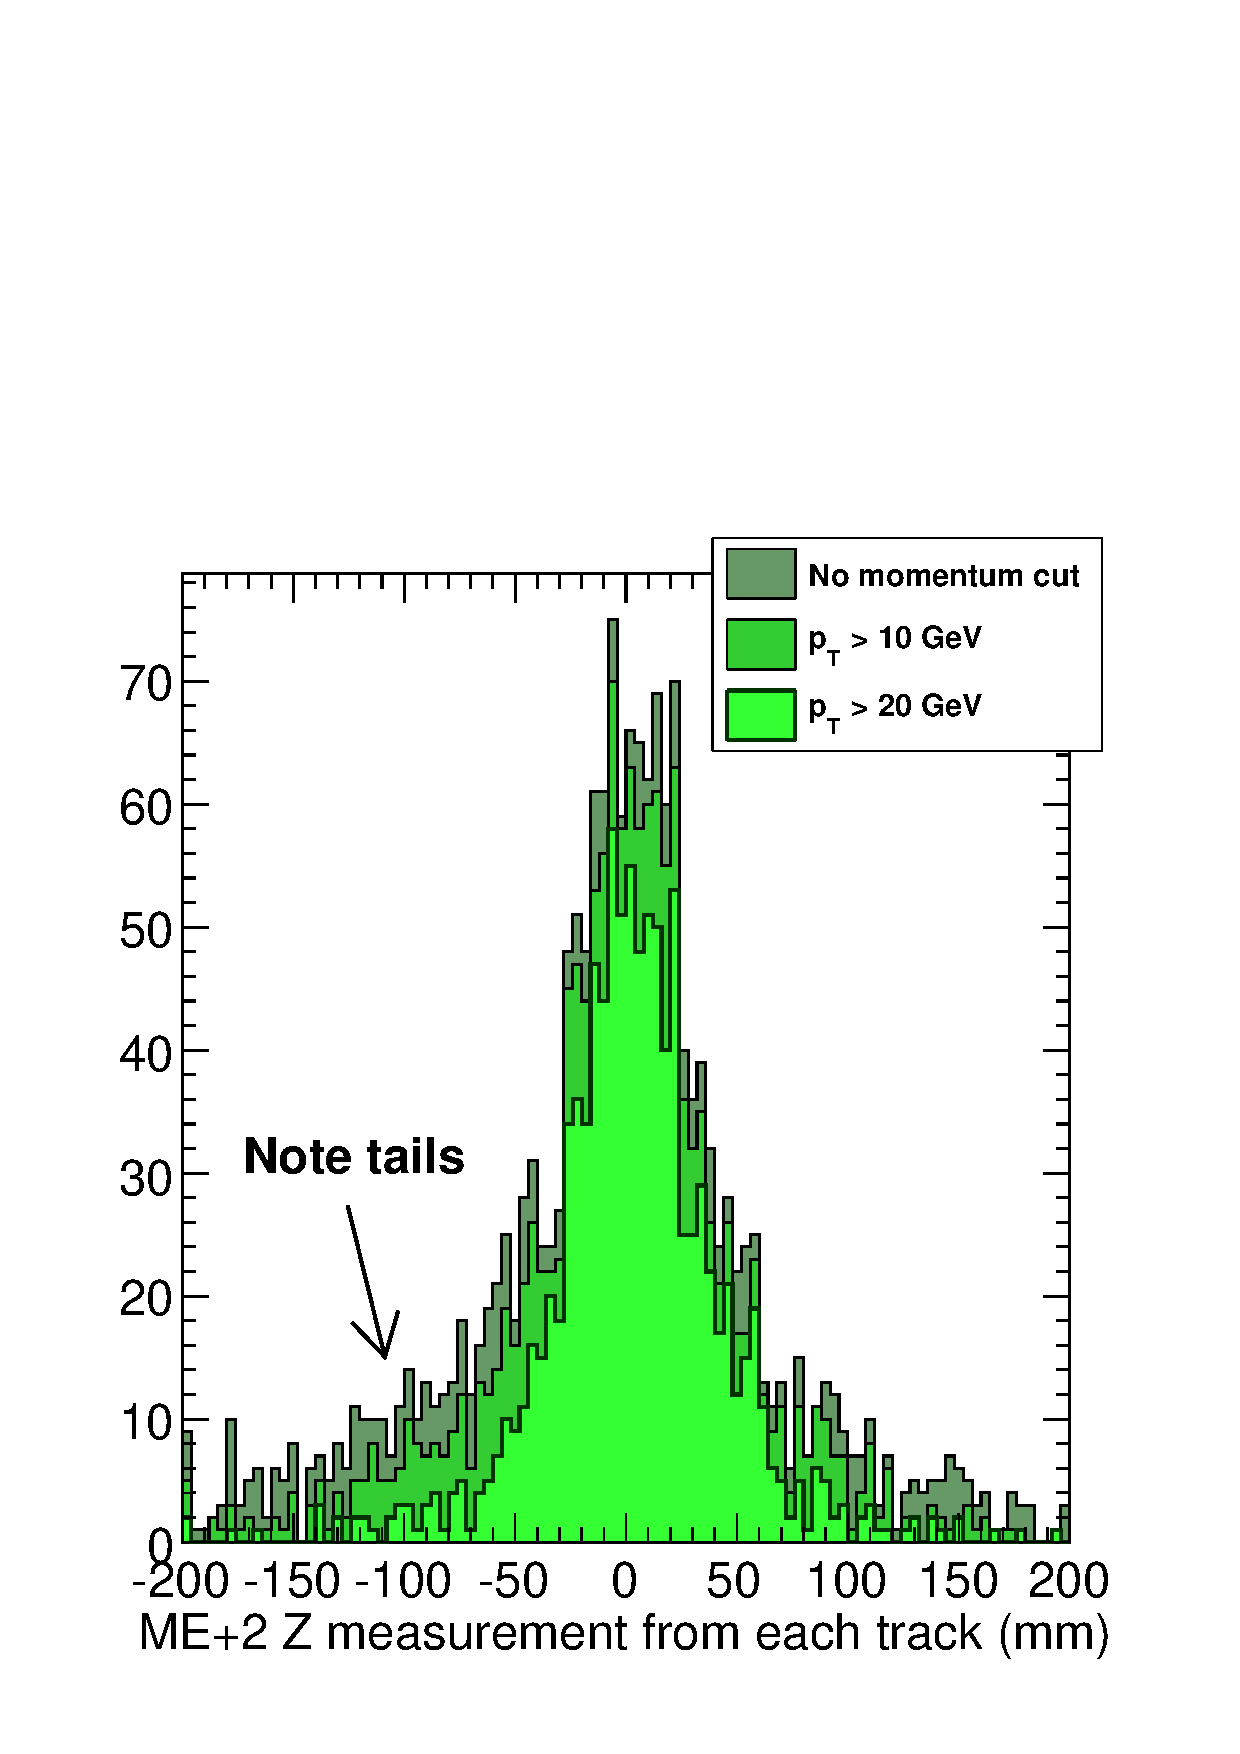
\includegraphics[width=\linewidth]{residuals_endcap.pdf}
\end{columns}

\begin{tabular}{p{0.5\linewidth} p{0.58\linewidth}}
\scriptsize Barrel wheel 0 & \scriptsize Endcap disk $+$2
\end{tabular}

\column{0.4\linewidth}
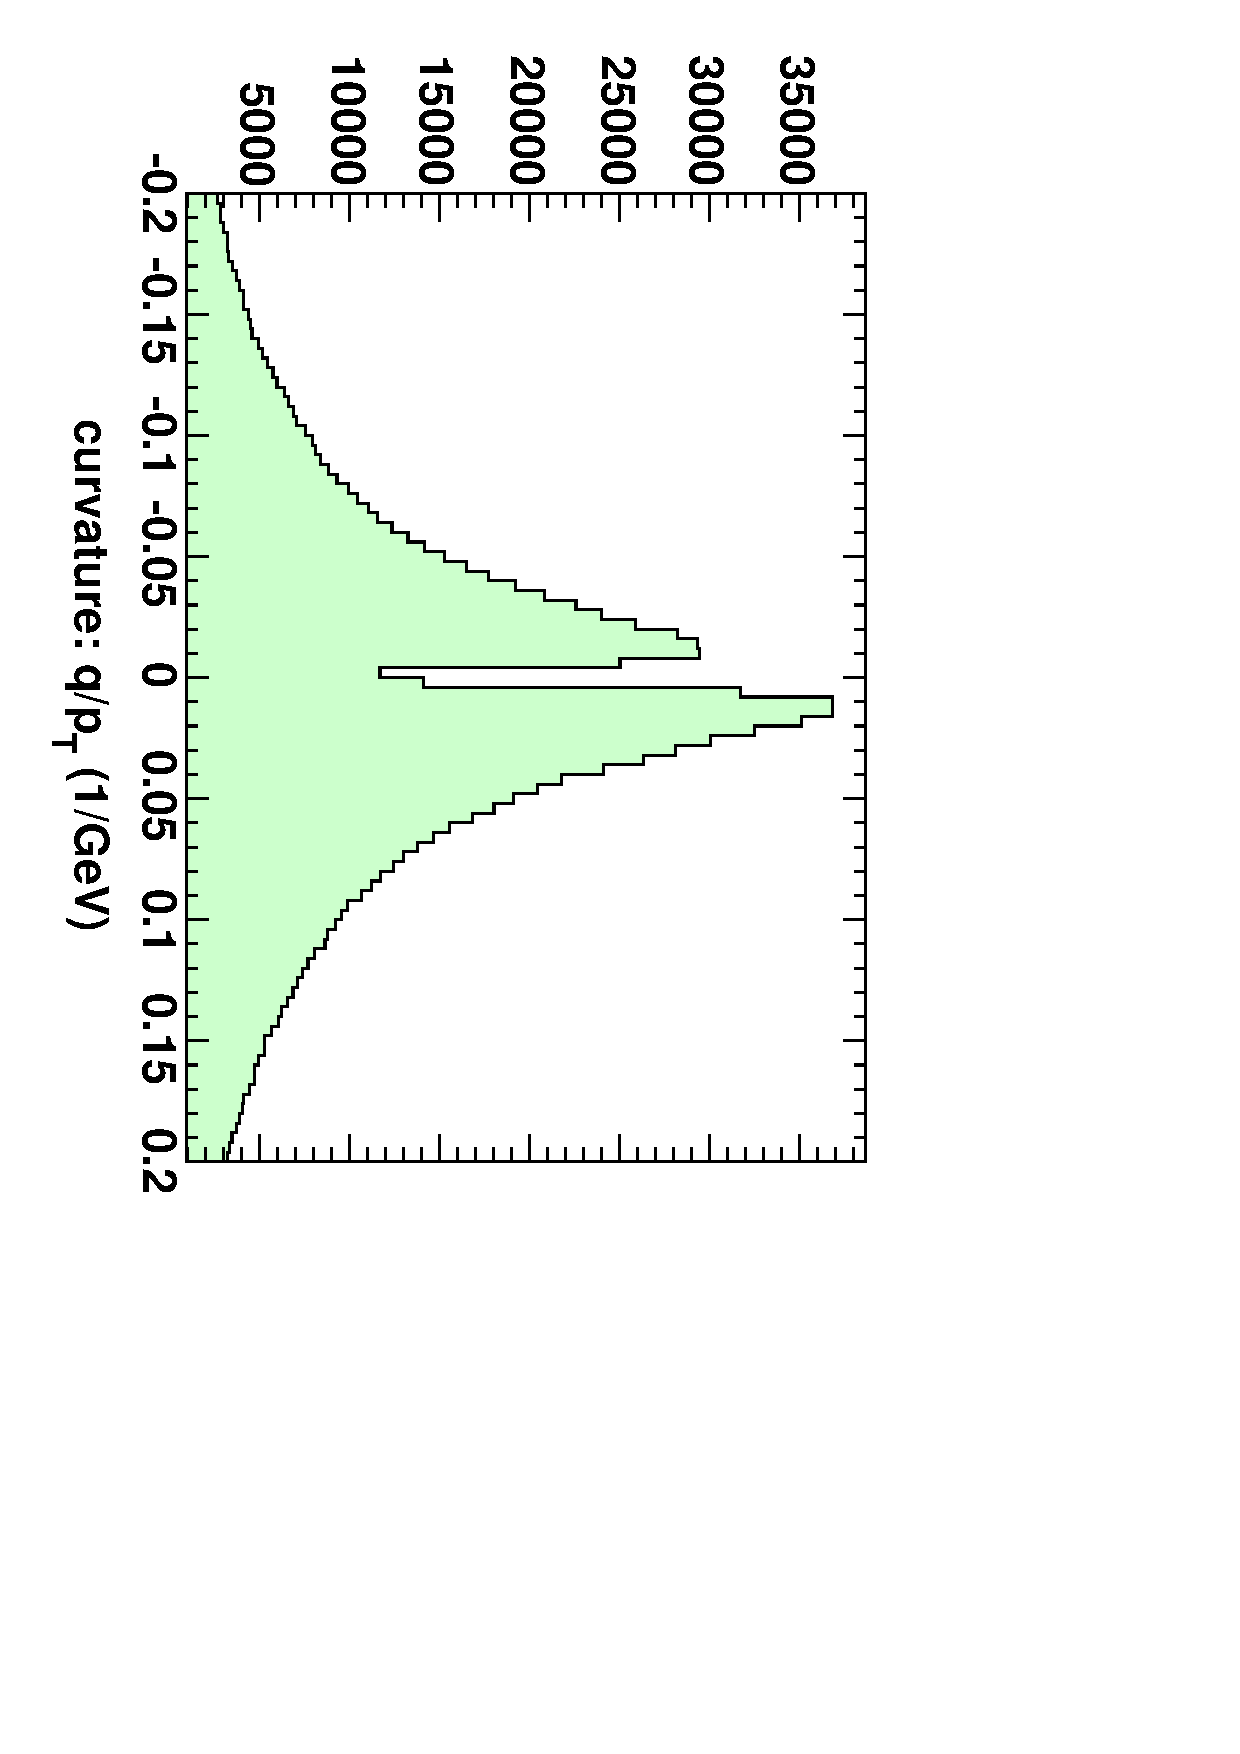
\includegraphics[height=\linewidth, angle=90]{qoverpt.pdf}

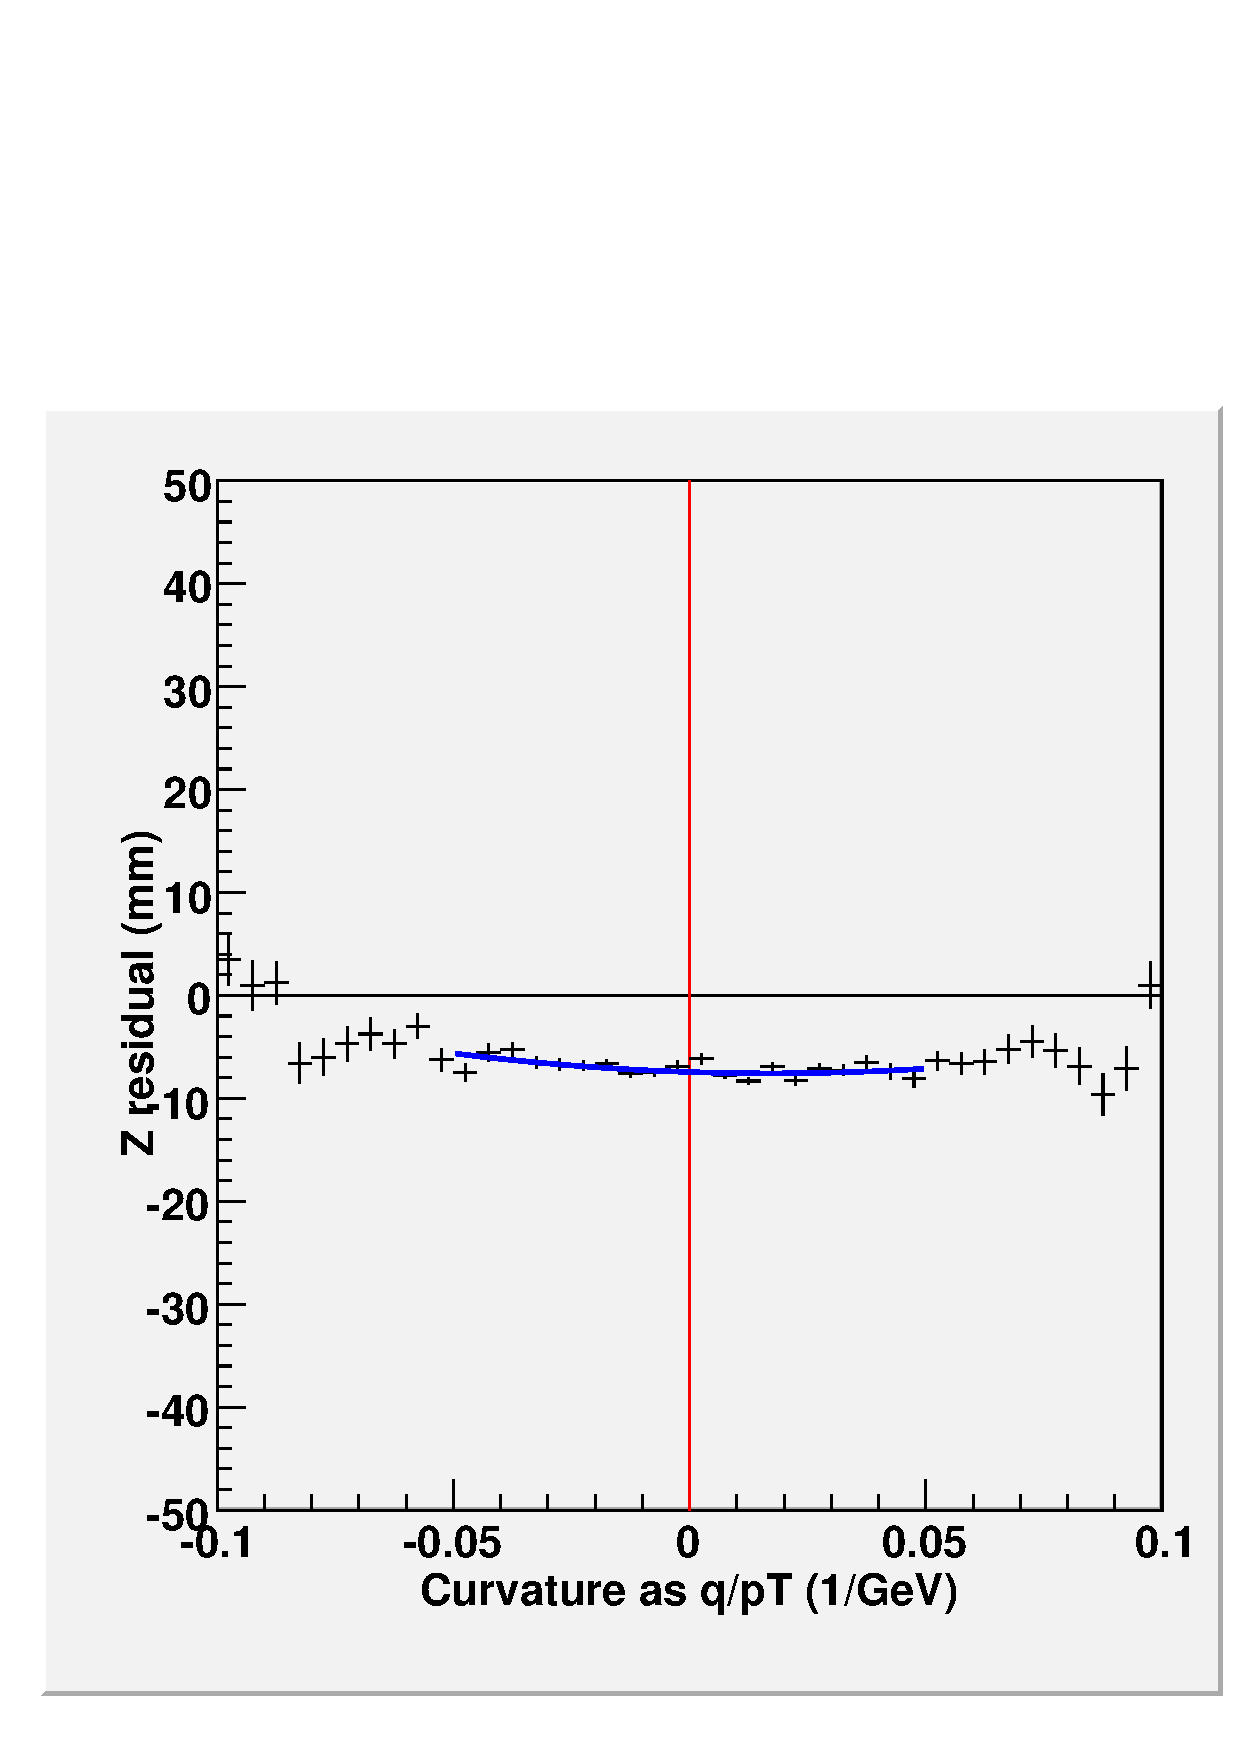
\includegraphics[width=\linewidth]{oprof_whm2_withcut.pdf}

\mbox{ } \hfill \scriptsize Barrel wheel $-$2 \hfill \mbox{ }

\end{columns}
\end{frame}

\begin{frame}
\frametitle{Twist around beamline}
\begin{columns}
\column{0.4\linewidth}
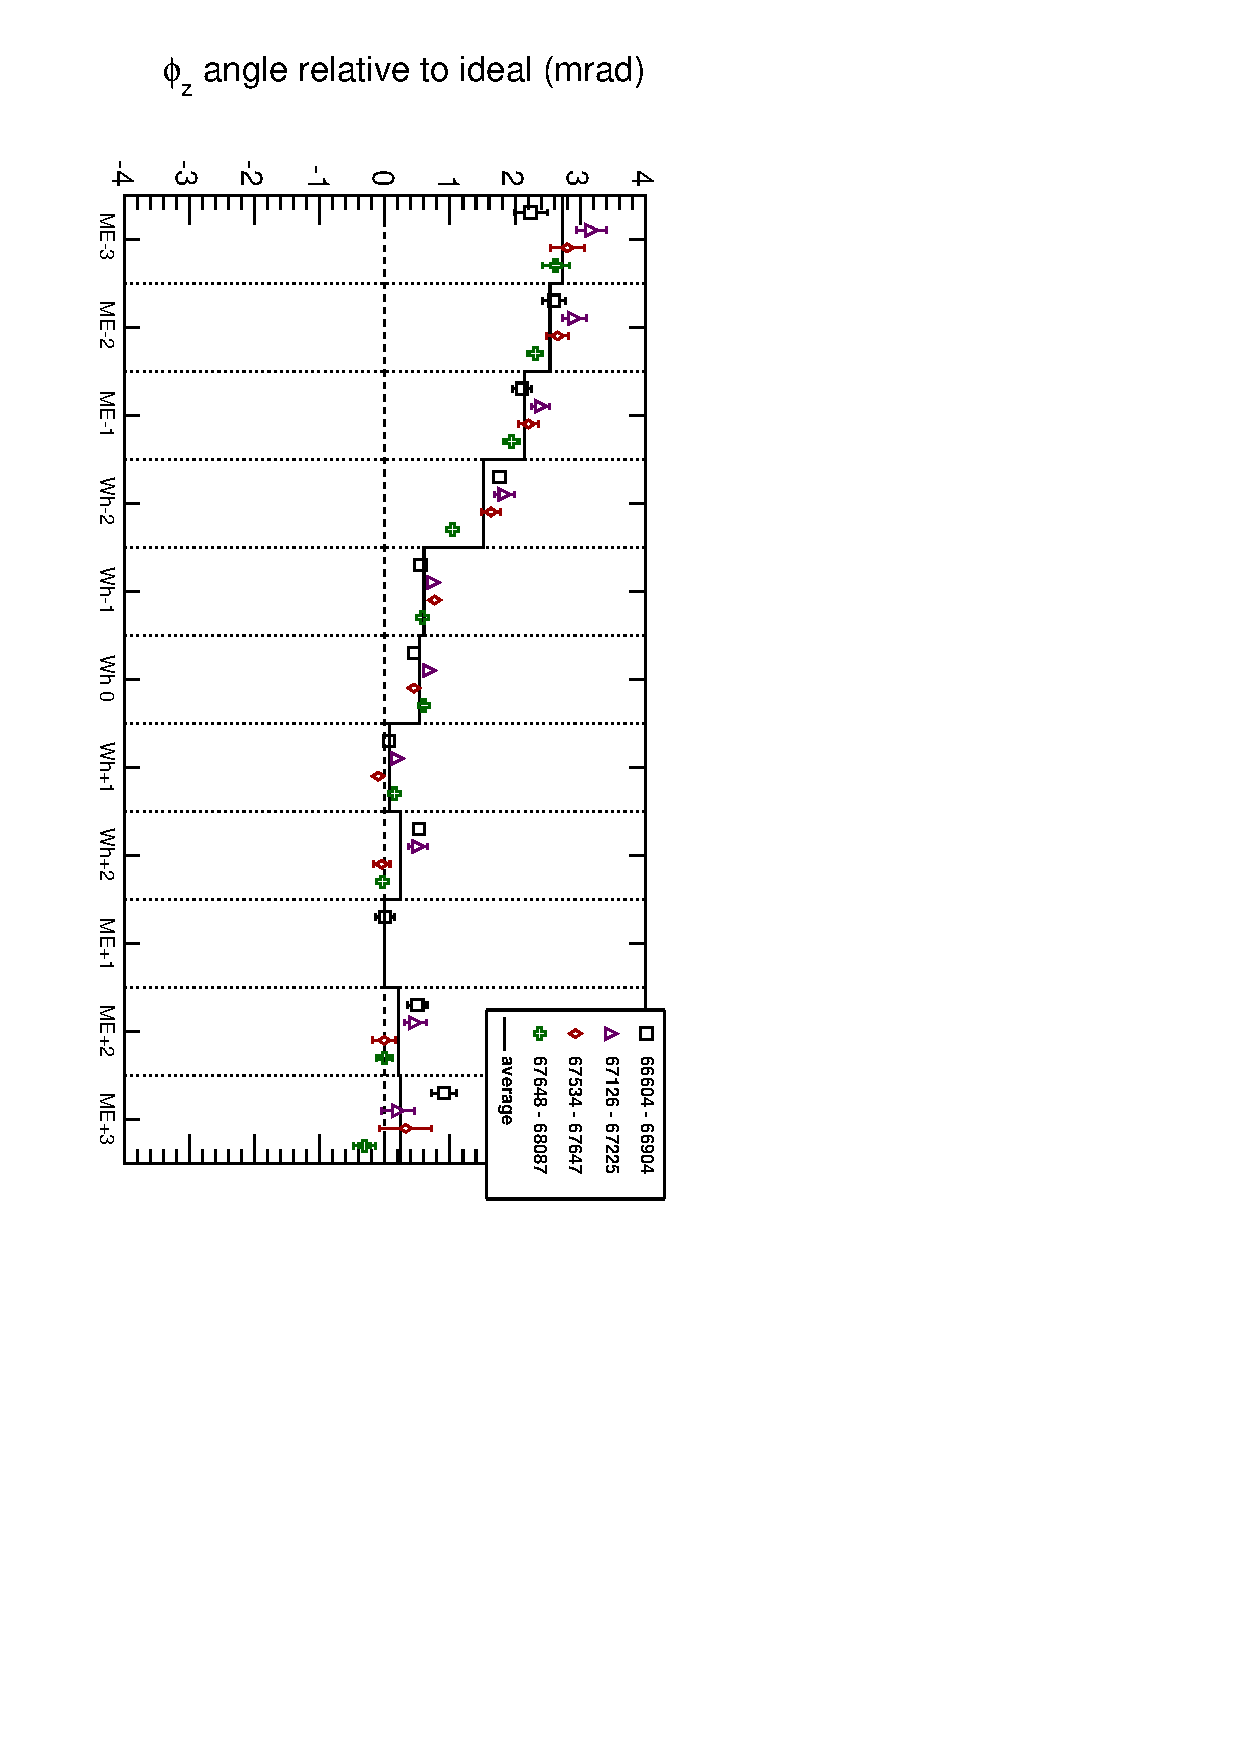
\includegraphics[height=1.25\linewidth, angle=90]{alierr_phiz.pdf}

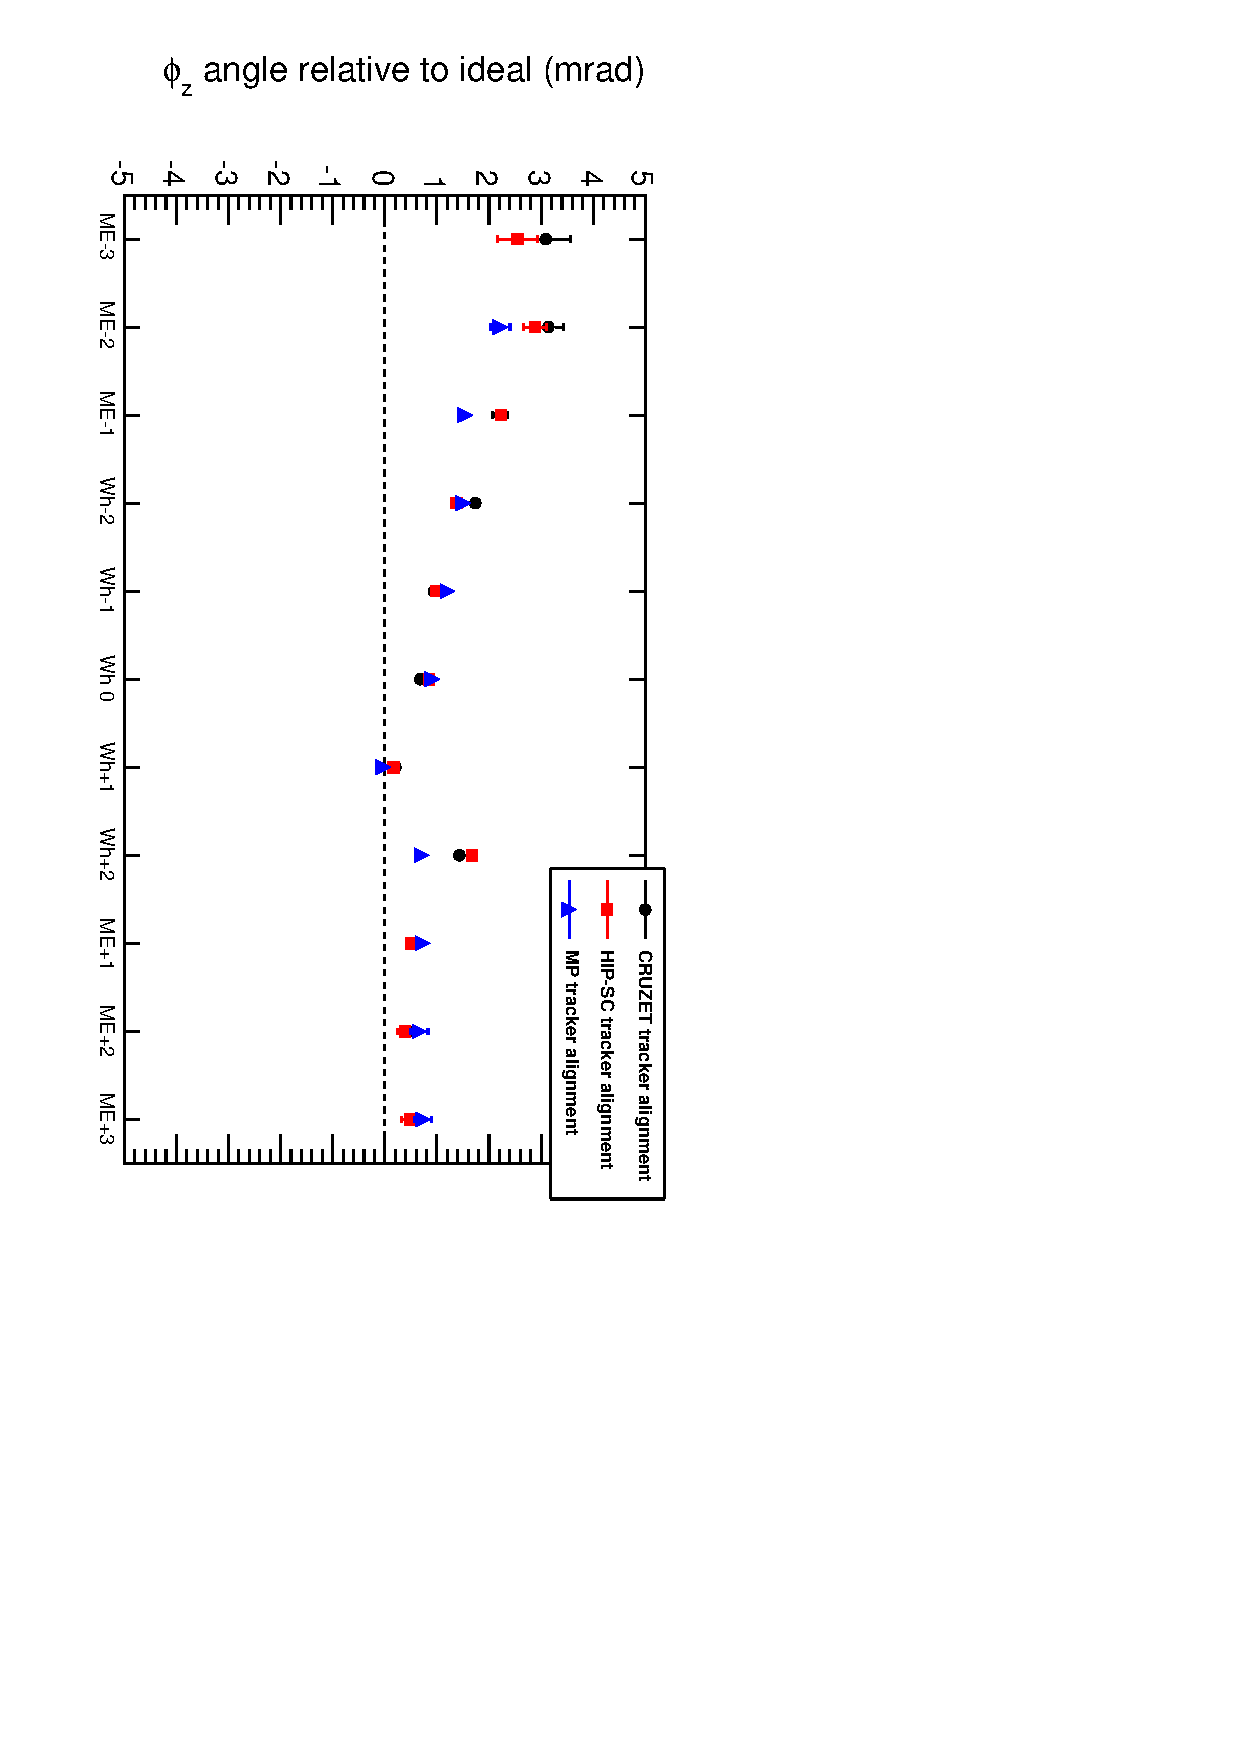
\includegraphics[height=1.25\linewidth, angle=90]{compare_tracker_alignment_phiz.pdf}

\mbox{ } \hfill 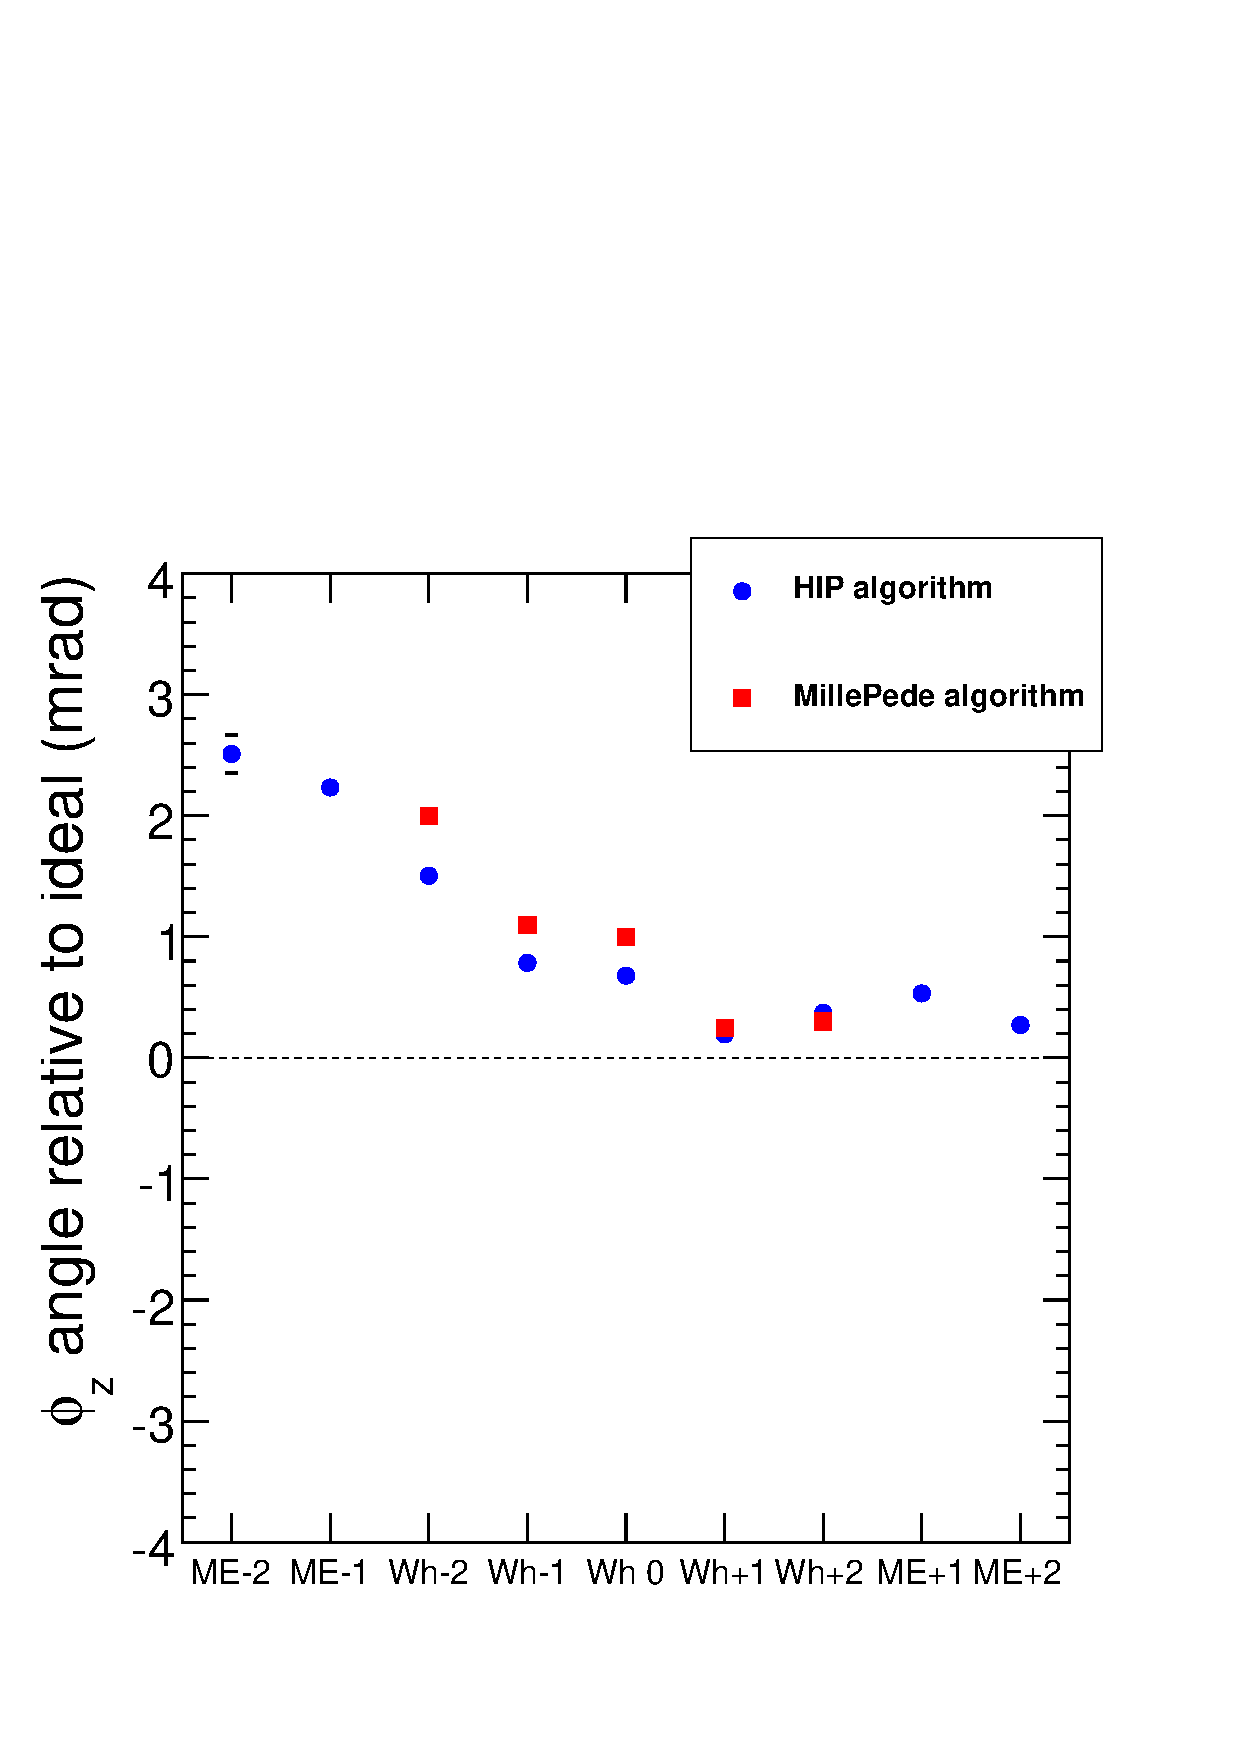
\includegraphics[width=0.625\linewidth]{hip_millepede_overlay_phiz.pdf} \hfill \mbox{ }

\column{0.5\linewidth}
\begin{itemize}
\item Aligned $\phi_z$ for all wheels/disks with
  the $q/p_T \to 0$ method

\vspace{-0.25 cm}
\begin{itemize}
\item effect of $\vec{B}$ error \mbox{is minimized\hspace{-1 cm}}
\end{itemize}

\item Observed a large (2.5~mrad) twist in the minus endcap 

\item Reproducible in

\vspace{-0.25 cm}
\begin{itemize}
\item all stable 3.8~T \mbox{runs (top plot)\hspace{-1 cm}}

\item all tracker \mbox{alignments (middle)\hspace{-1 cm}}

\item both algorithms \mbox{(bottom)\hspace{-1 cm}}
\end{itemize}

\item $\vec{B}=0$ photogrammetry \mbox{constrains\hspace{-0.5 cm}} $\phi_z$ differences at 0.5~mrad

\item Could this be

\vspace{-0.25 cm}
\begin{itemize}
\item real twisting as \mbox{$\vec{B} \to 3.8$~T?\hspace{-1 cm}}
\item an artifact of \mbox{external bias?\hspace{-0.5 cm}}
\end{itemize}

\end{itemize}

\vspace{0.25 cm}
\begin{columns}
\column{1.2\linewidth}
\tiny HIP: J.\ Pivarski, A.\ Safonov

MillePede: P.\ Martinez, F.\ Matorras, J.\ Fernandez, A.\ Calderon
\end{columns}
\end{columns}
\end{frame}

\begin{frame}
\frametitle{Apparently, a little of both}
\begin{itemize}
\item Divide wheels/disks into smaller bins by plotting as a function of $z$
\begin{itemize}
\item obvious discontinuities at wheel boundaries are real \mbox{misalignments\hspace{-1 cm}}
\item slope within wheels is external bias
\end{itemize}
\end{itemize}

\begin{columns}
\column{1.1\linewidth}
\begin{tabular}{c c}
\scriptsize from the HIP group & \scriptsize from the MillePede group \\
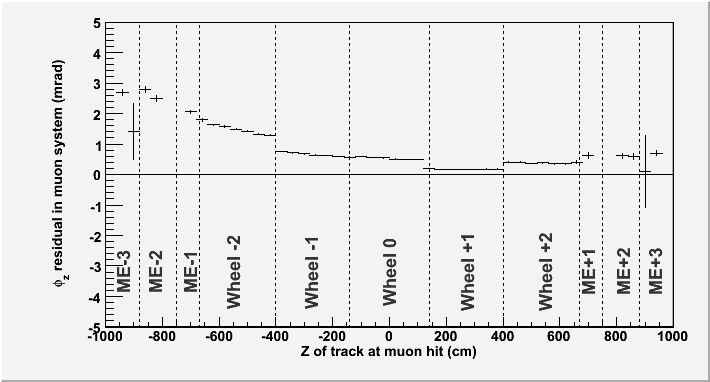
\includegraphics[height=3.4 cm]{phiresid_from_muon.png} & 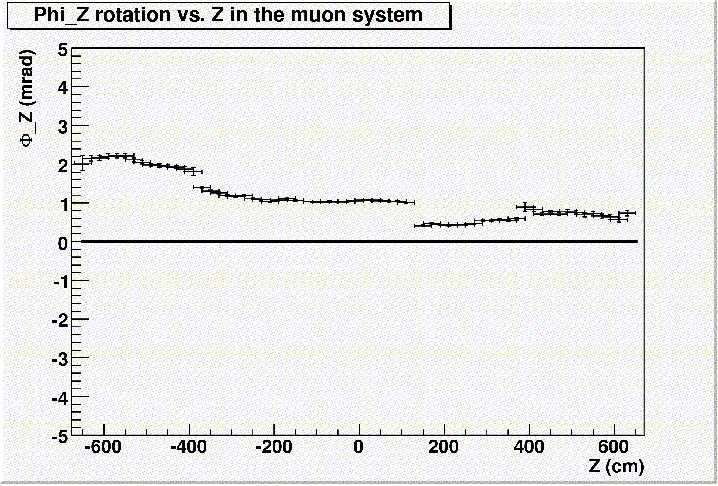
\includegraphics[height=3.4 cm]{phiresid_vs_z_millepede.png}
\end{tabular}
\end{columns}

\begin{itemize}
\item Possible sources of external bias
\begin{itemize}\setlength{\itemsep}{0.1 cm}
\item global distortions in tracker, extrapolated to muon system
\item propagation errors?
\item \sout{$\vec{B}$ errors?} ($|\vec{p}| > 40$~GeV in the HIP plot)
\end{itemize}
\end{itemize}
\end{frame}

\begin{frame}
\frametitle{Invert problem: align tracker?}

\vspace{0.25 cm}
\begin{columns}
\column{0.4\linewidth}
\textcolor{darkblue}{Normal muon alignment}

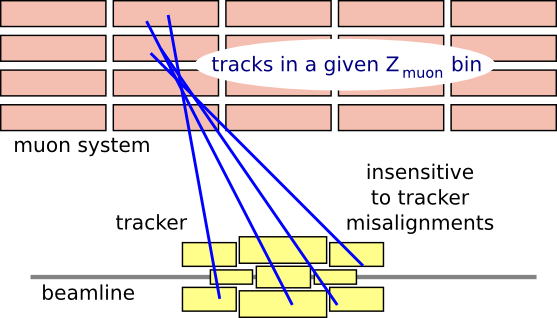
\includegraphics[width=\linewidth]{globalMuons_vsmuon.png}

\column{0.4\linewidth}
\textcolor{darkblue}{Tracker study}

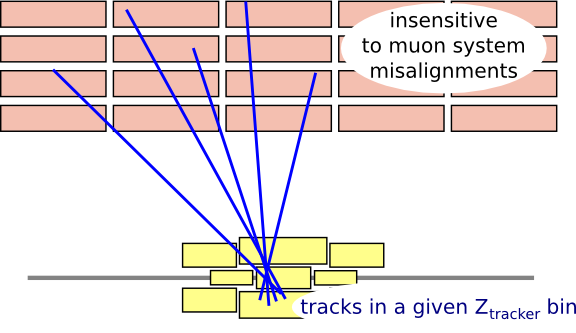
\includegraphics[width=\linewidth]{globalMuons_vstracker.png}
\end{columns}

\vspace{0.1 cm}
\begin{columns}
\column{0.6\linewidth}
\begin{itemize}\setlength{\itemsep}{0.25 cm}
\item Plot muon $\phi_z$ residuals vs.\ \mbox{$Z_{\mbox{\scriptsize tracker}}$ (black)\hspace{-1 cm}}
\begin{itemize}
\item broad distribution of entrance angles effectively averages over
  the muon system
\end{itemize}

\item Slope (0.2~mrad across TOB) may indicate a twist in the tracker
\item Zijin Guo added a tracker twist \mbox{by hand\hspace{-0.5 cm}} (0.6~mrad, blue): \mbox{easily observed\hspace{-1 cm}}
\end{itemize}

\column{0.4\linewidth}
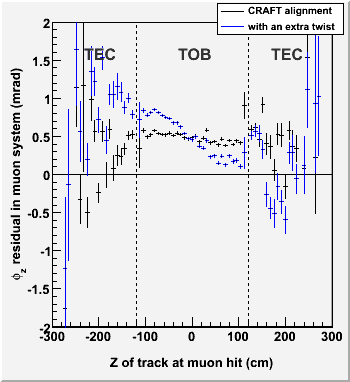
\includegraphics[width=\linewidth]{phiresid_from_tracker_outer_twist2.png}
\end{columns}
\end{frame}

\begin{frame}
\frametitle{Expansion in $z$}

\begin{columns}
\column{0.4\linewidth}
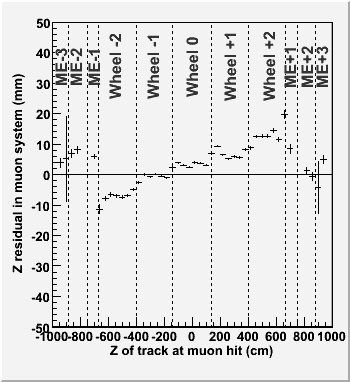
\includegraphics[width=\linewidth]{zresid_from_muon.png}

\column{0.6\linewidth}
GlobalMuons think that the muon system is {\it wider} than ideal geometry

\vspace{-0.1 cm}
\begin{itemize}\setlength{\itemsep}{-0.05 cm}
\item $+$14~mm across barrel (0.2\%)
\item $\vec{B}$ ought to {\it compress} in $z$
\item perhaps ideal isn't intended to represent $\vec{B}=0$, and this is compression relative to true $\vec{B}=0$?
\end{itemize}

\mbox{ }
\end{columns}

\vspace{-0.75 cm}
\begin{columns}
\column{0.6\linewidth}

\vspace{0.75 cm}
Is muon alignment affected by tracker $z$-expansion?
\begin{itemize}
\item No: muon residuals can't resolve a plausible
  $z$-expansion (black vs.\ blue: 0.1\% tracker stretch)

\item But we can see large displacements of TEC relative to TOB (discontinuity)
\end{itemize}

\column{0.4\linewidth}
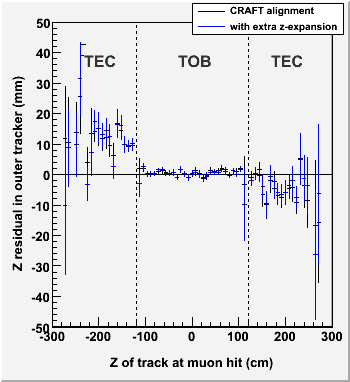
\includegraphics[width=\linewidth]{resid_from_tracker_outer_zexpand.png}

\end{columns}
\end{frame}

\begin{frame}
\frametitle{Study of tracker $z$ alignment}

\begin{itemize}
\item Select parts of the tracker by cutting on $R_{PCA}$ and by removing outer tracker hits from refit (to highlight inner tracker)
\end{itemize}

\vfill
\begin{columns}
\column{0.25\linewidth}
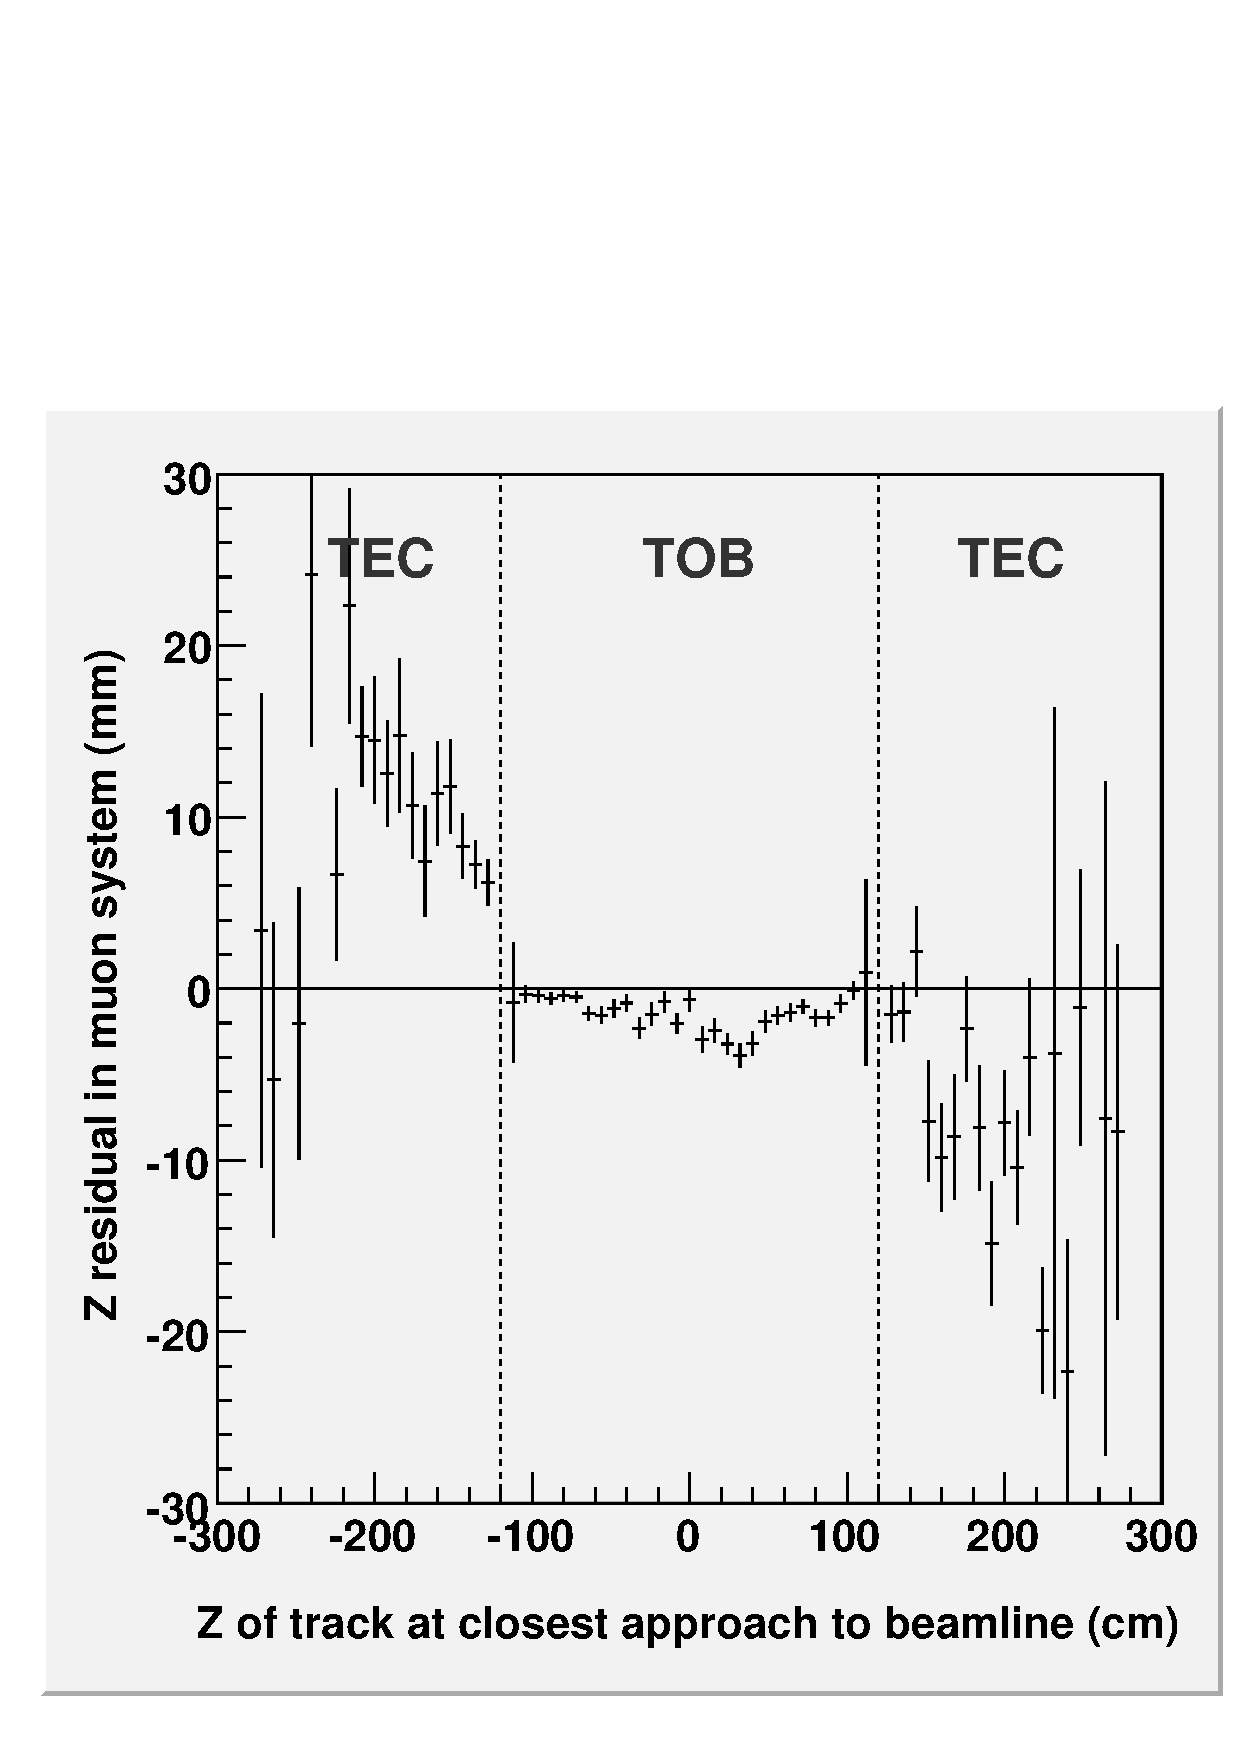
\includegraphics[width=\linewidth]{zresid_from_tracker_outerbottom.pdf}

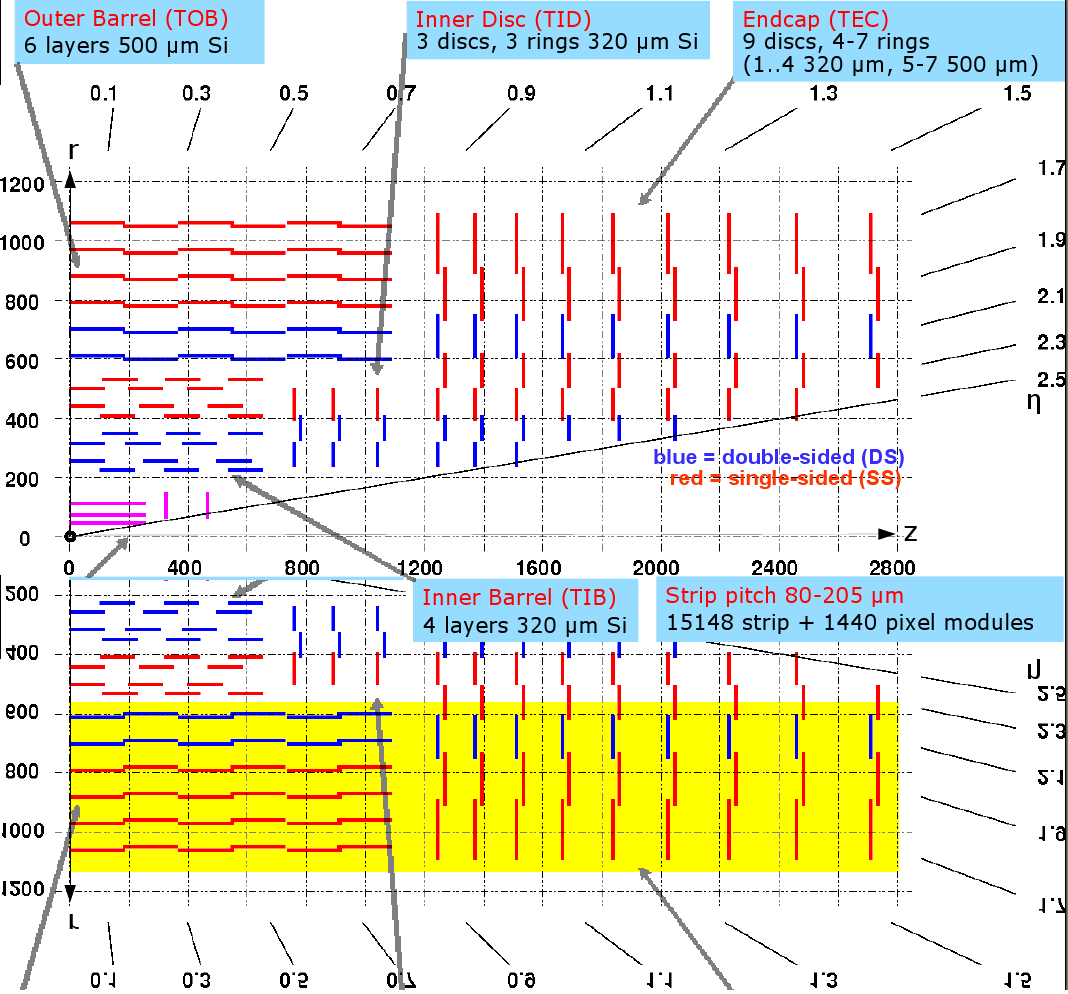
\includegraphics[width=\linewidth]{tracker_map_outerbottom.png}

\column{0.25\linewidth}
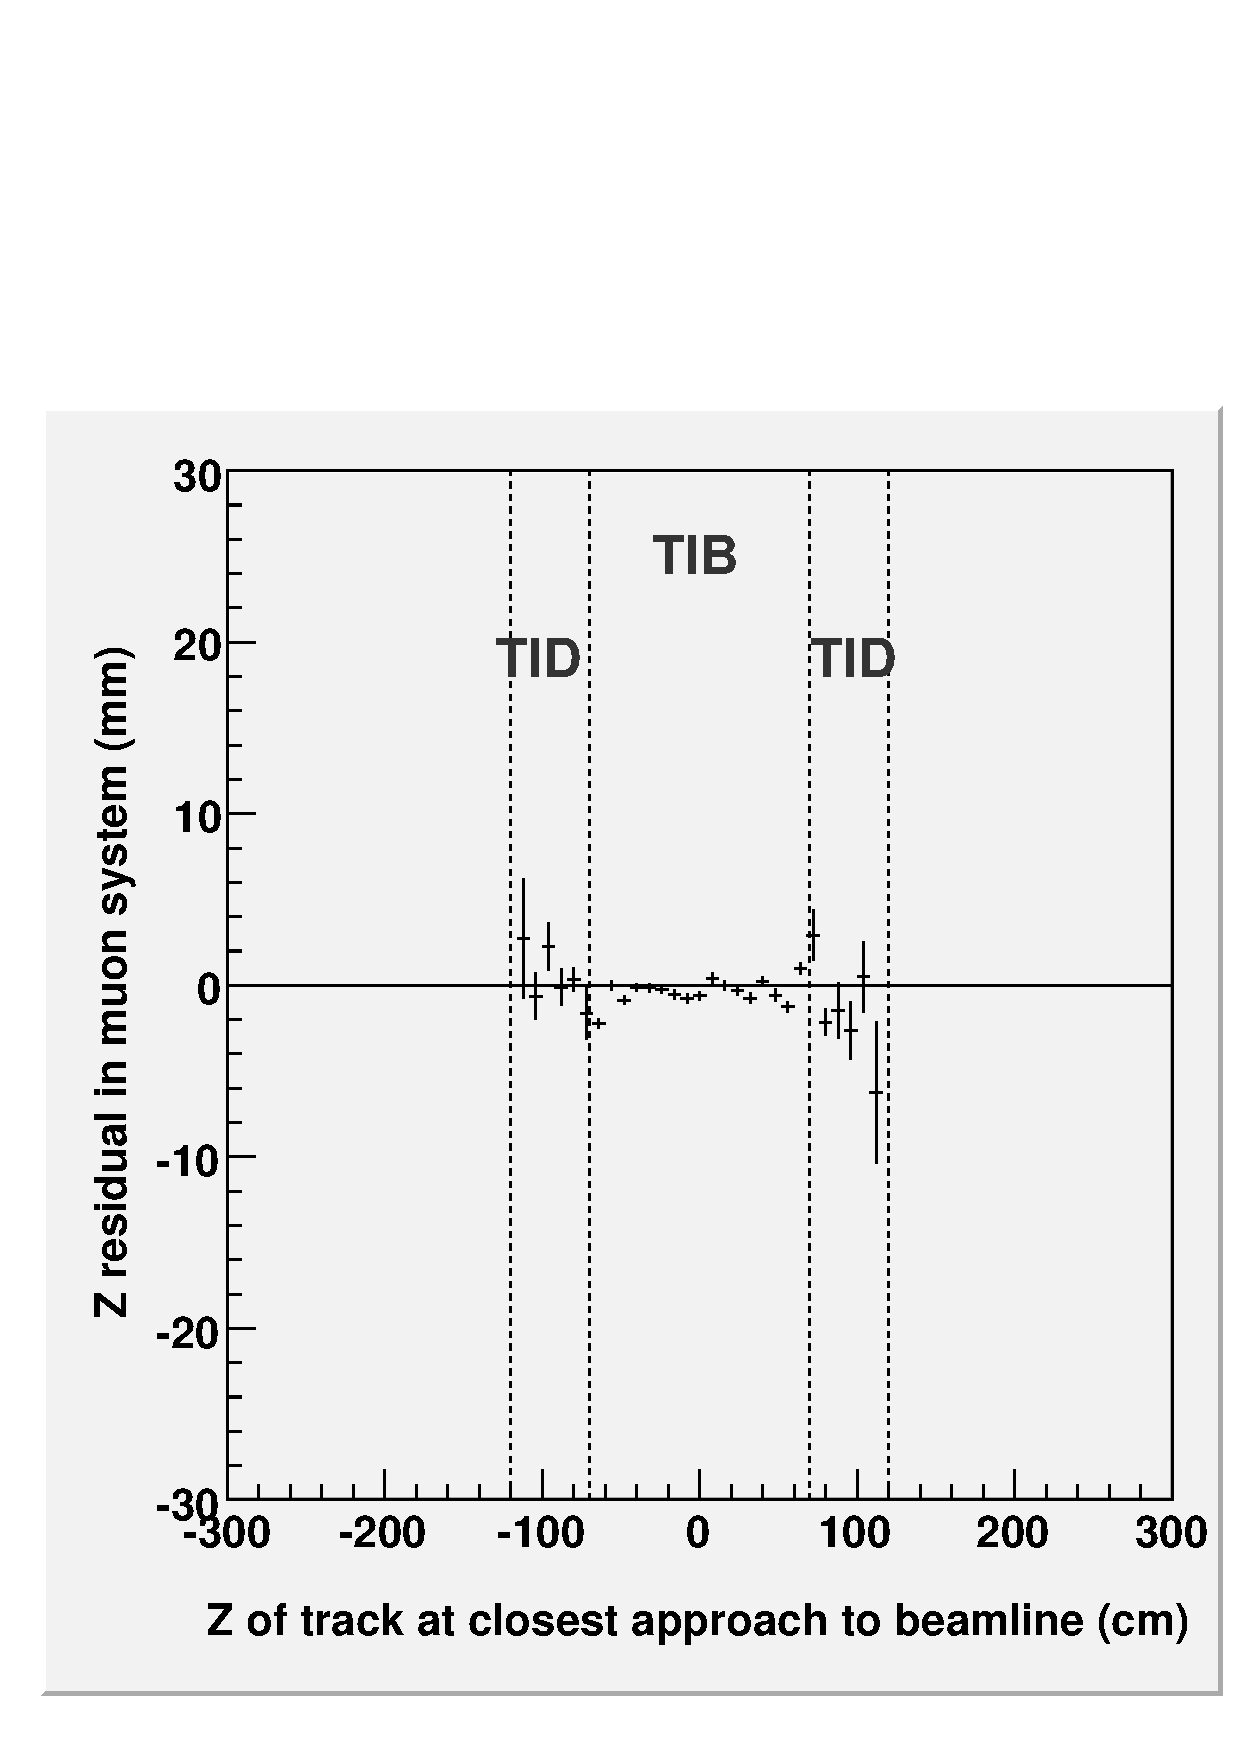
\includegraphics[width=\linewidth]{zresid_from_tracker_innerbottom.pdf}

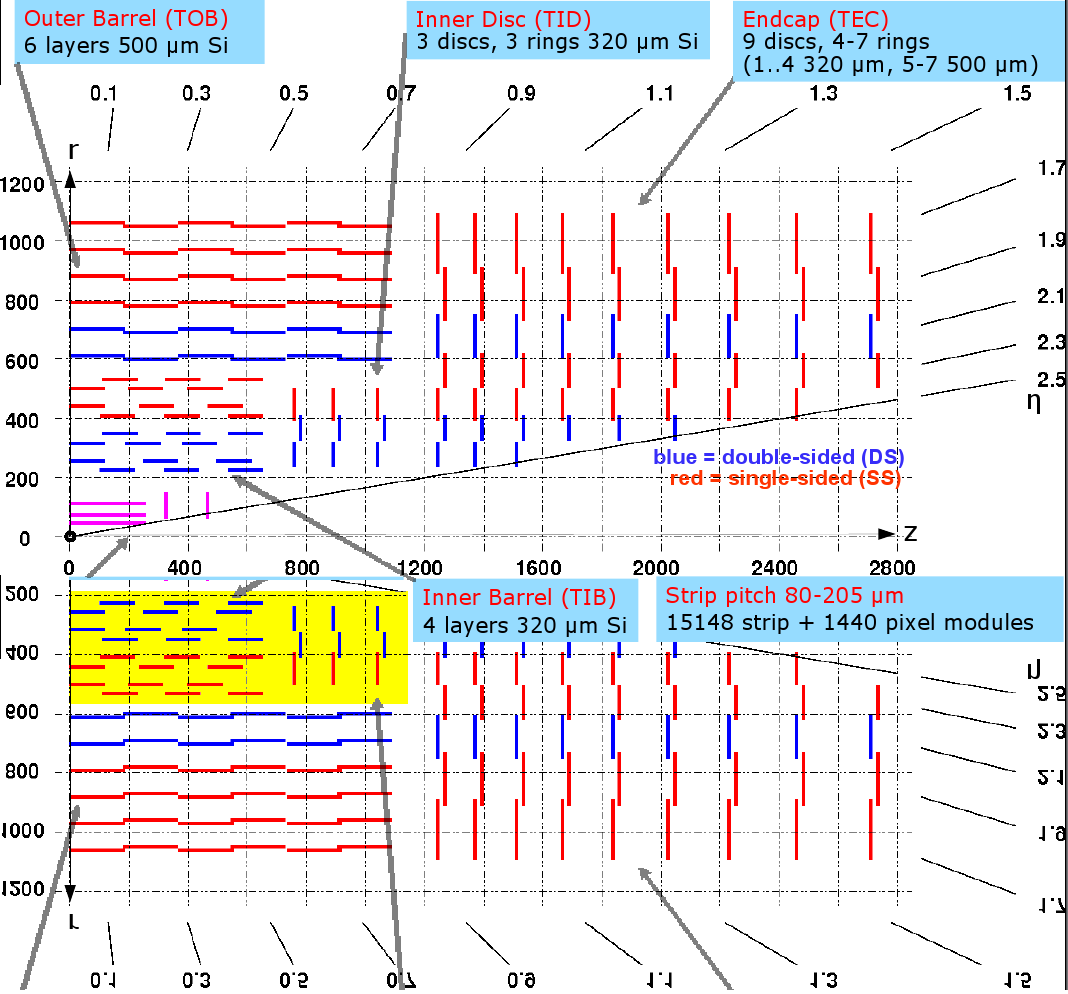
\includegraphics[width=\linewidth]{tracker_map_innerbottom.png}

\column{0.25\linewidth}
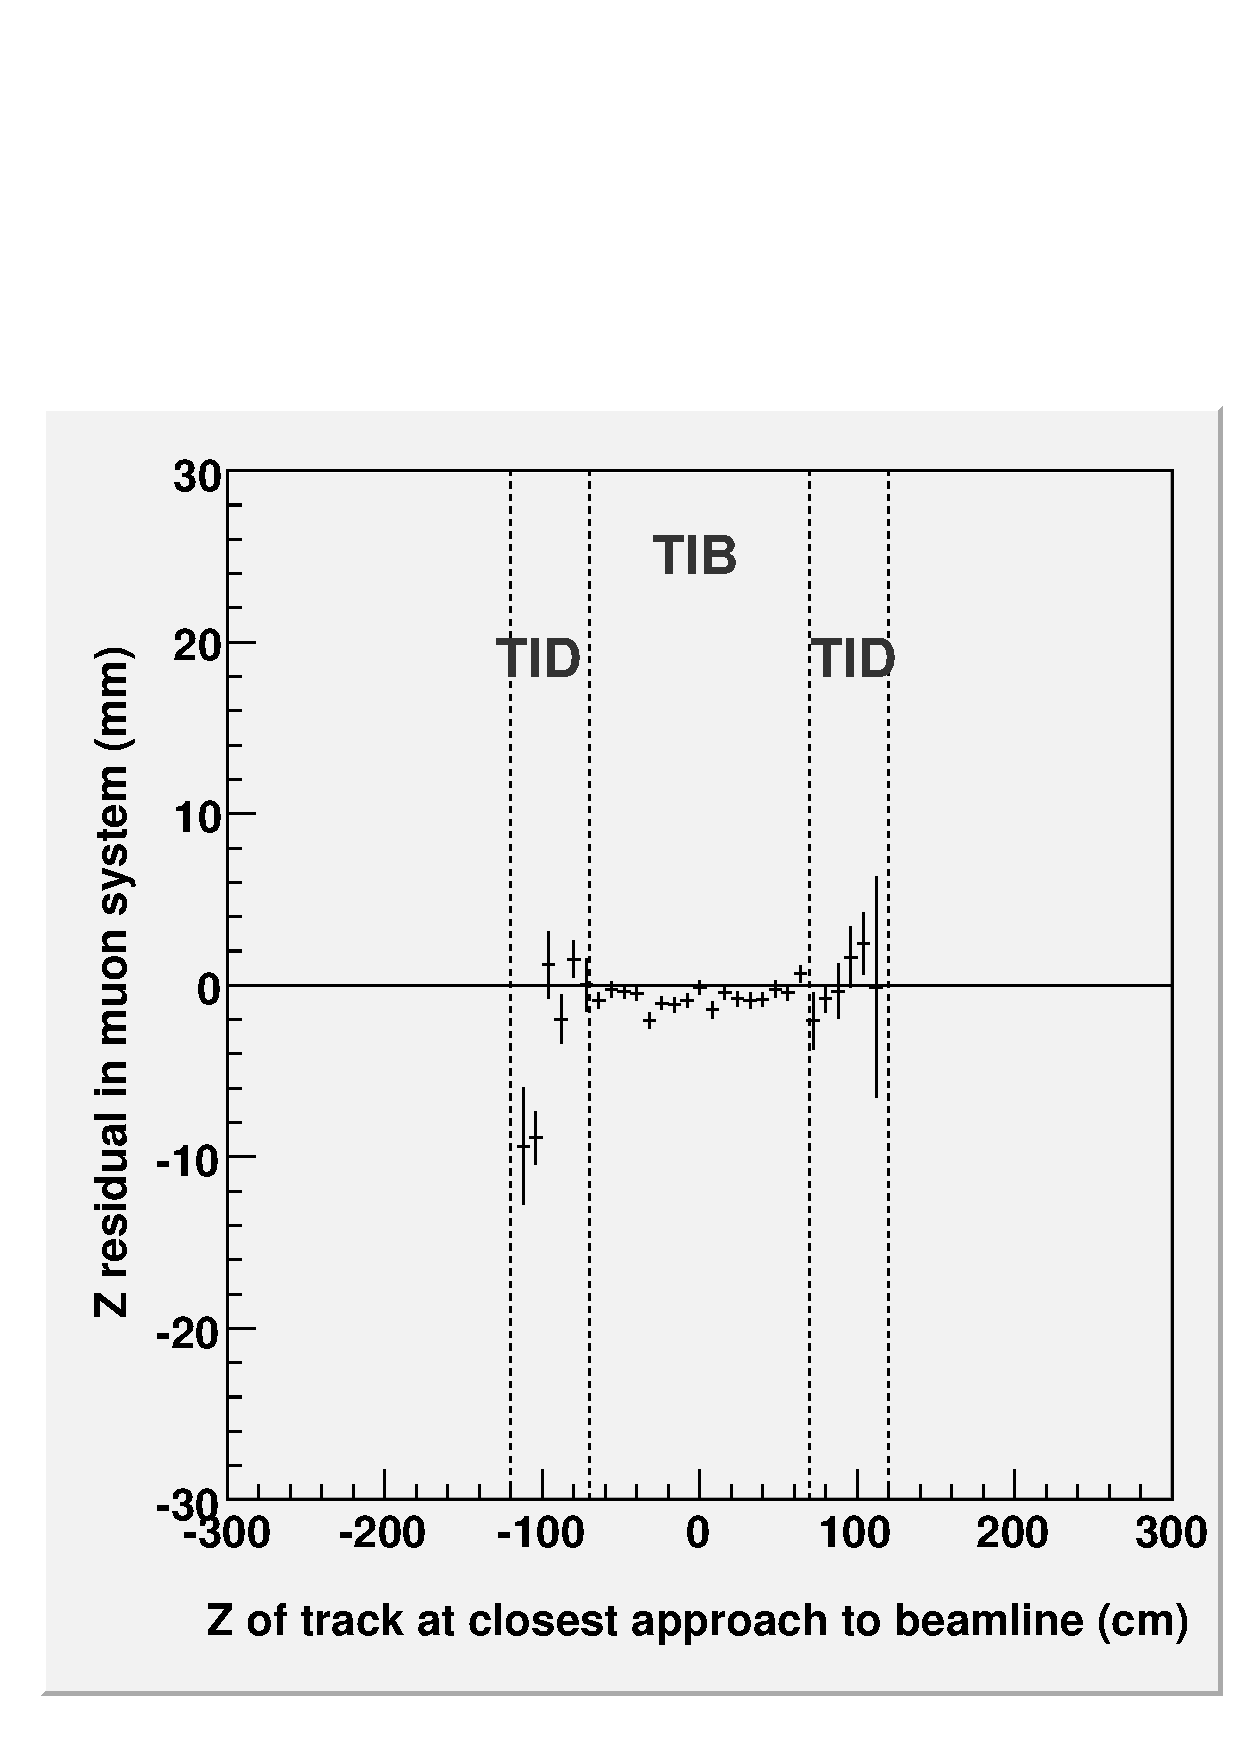
\includegraphics[width=\linewidth]{zresid_from_tracker_innertop.pdf}

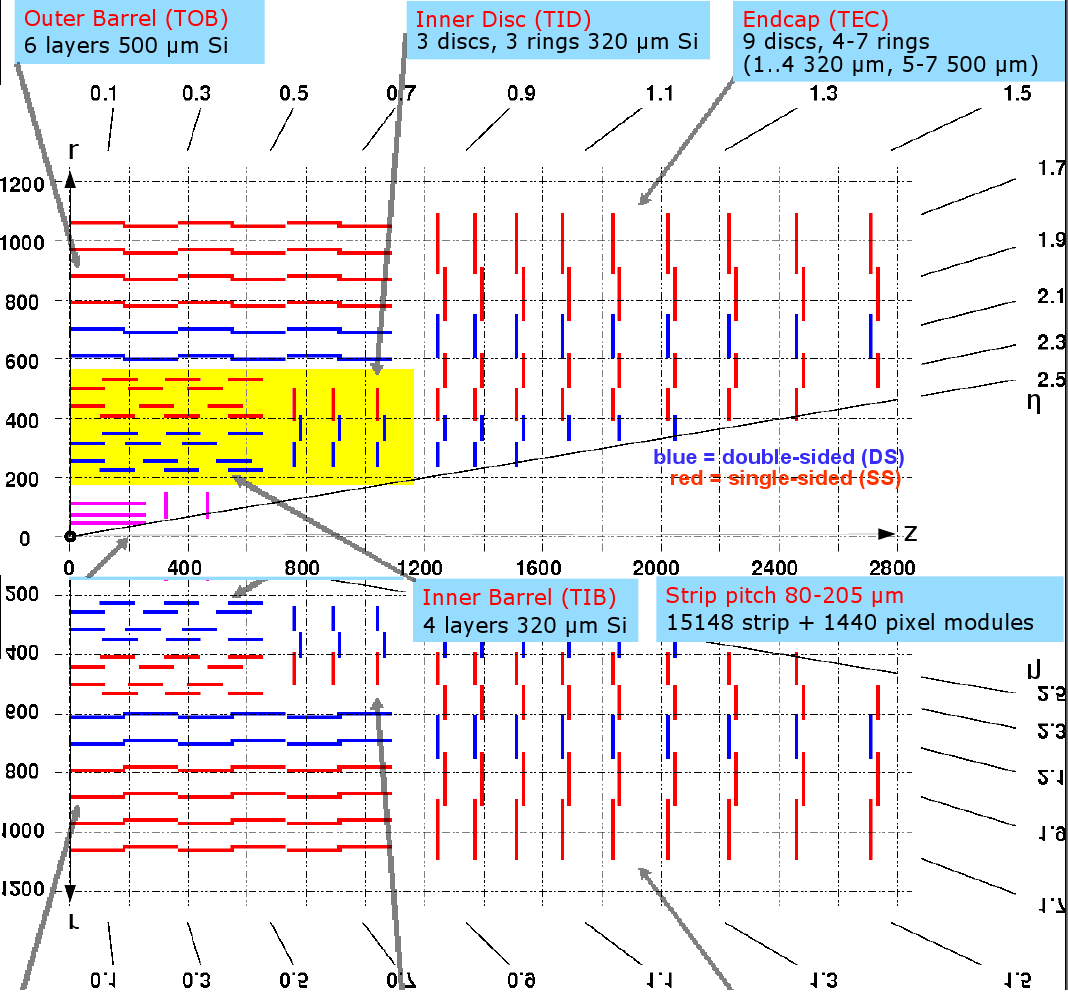
\includegraphics[width=\linewidth]{tracker_map_innertop.png}

\column{0.25\linewidth}
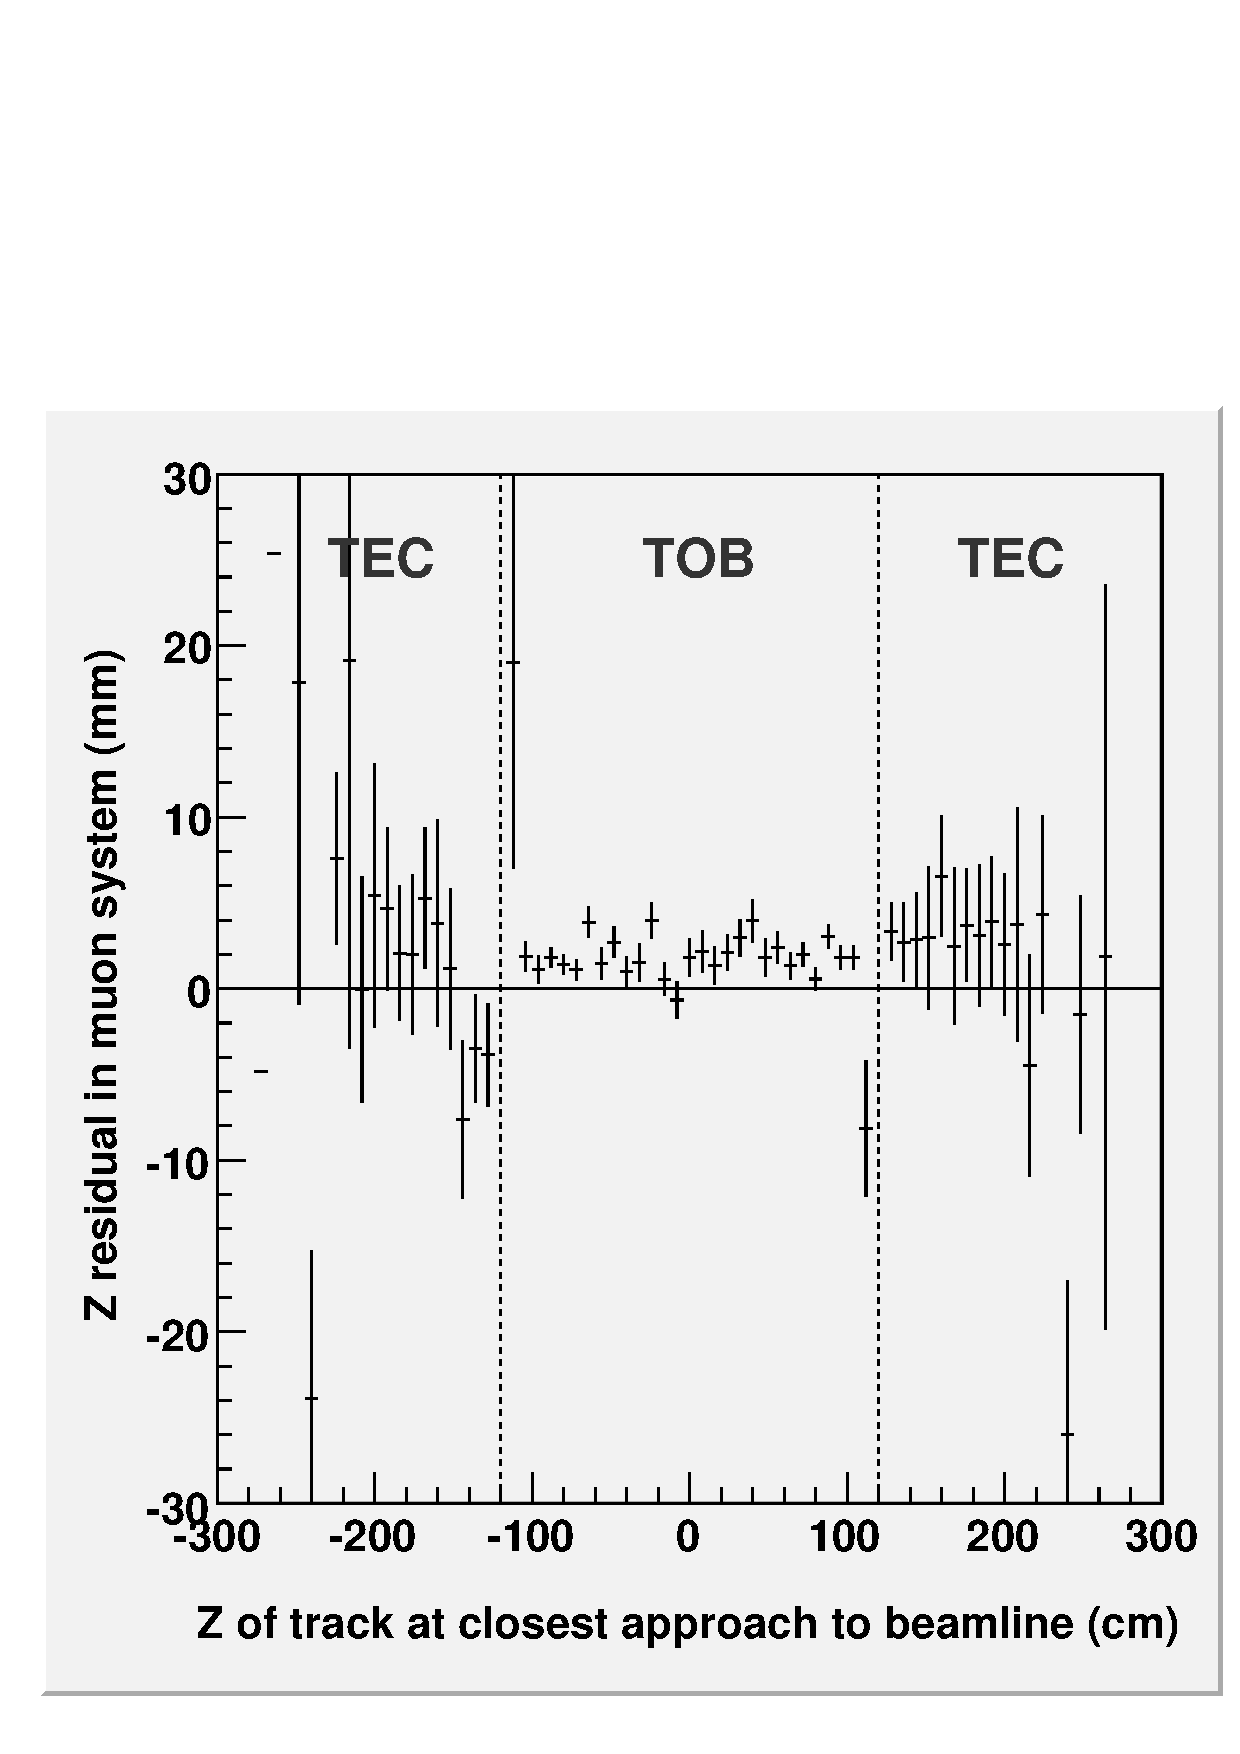
\includegraphics[width=\linewidth]{zresid_from_tracker_outertop.pdf}

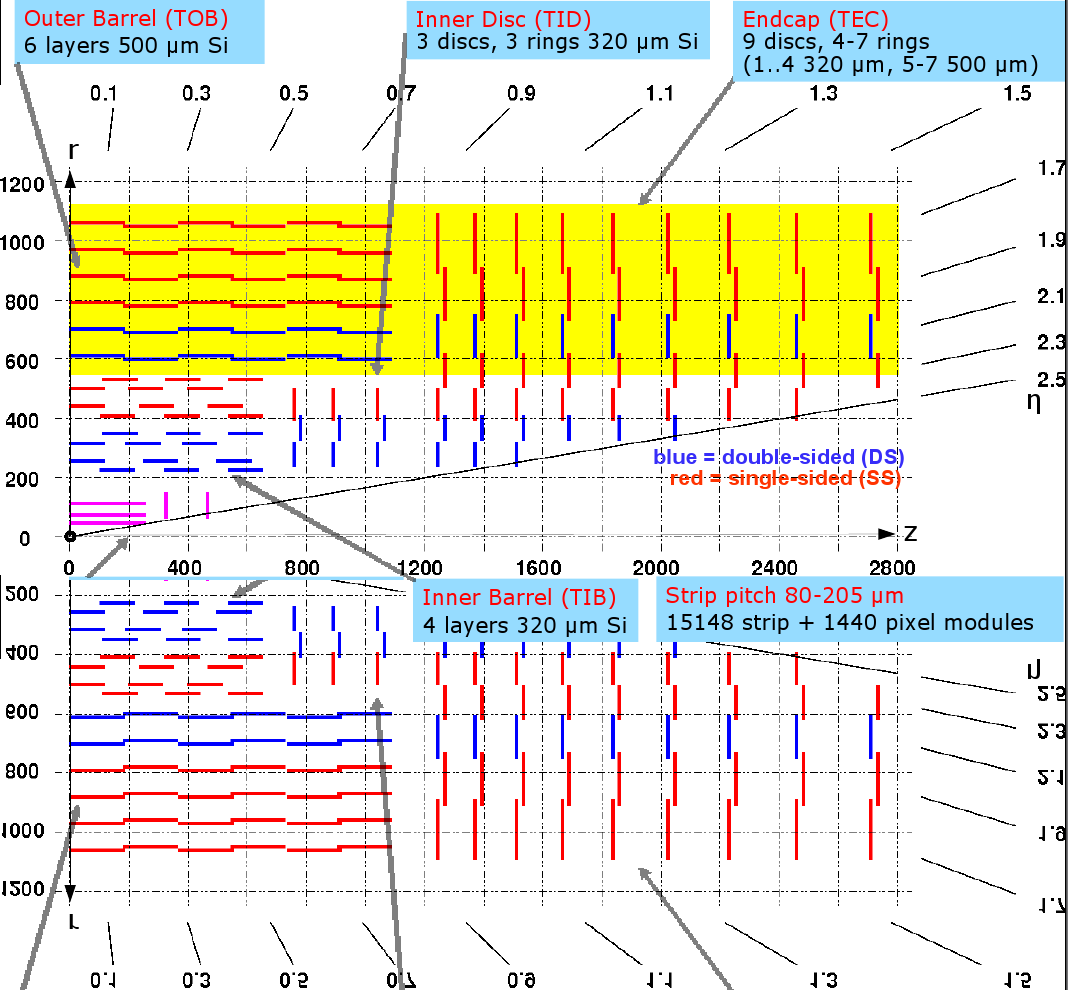
\includegraphics[width=\linewidth]{tracker_map_outertop.png}
\end{columns}
\end{frame}

\begin{frame}
\frametitle{Conclusions}
\begin{itemize}\setlength{\itemsep}{0.5 cm}
\item CSC Alignment: achieved 300~$\mu$m resolution with minutes of beam-halo data
\begin{itemize}
\item verified by an independent measurement (photogrammetry)
\item predicted a 10~$\mu$m correction in chamber geometry
\item can align layers with a similar technique
\end{itemize}

\item Wheel/disk alignment
\begin{itemize}
\item many cross-checks are available in this huge dataset
\item a significant part of the twist we saw was real
\item is ideal-geometry barrel more compressed than real barrel at $\vec{B} = 3.8$~T?
\end{itemize}

\item Global CMS alignment
\begin{itemize}
\item muon system can provide feedback to tracker; we could iterate alignment
\end{itemize}

\end{itemize}
%% \hspace{-0.83 cm} \textcolor{darkblue}{\Large Outline2}
\label{numpages}
\end{frame}

\end{document}
